\documentclass[11pt, article, twoside,openright]{book}
% For math  
\usepackage{amsmath}
% For images
\usepackage{graphicx}  
\usepackage{caption}  
\usepackage{subcaption}
% Encoding of the text  
\usepackage[T1]{fontenc}
\usepackage{verbatim}
% No numbering of Chapter pages
\usepackage{titlesec}
\assignpagestyle{\chapter}{empty}
% For \definecolor
\usepackage{xcolor}        
% For \hypersetup
\usepackage{hyperref}      
% To have numbers on subsubsections
\setcounter{secnumdepth}{3}

\usepackage{appendix}
\usepackage[backend=biber,  
style=phys,  
sorting=none,  
giveninits=true,  
maxnames=2,  
minnames=1]{biblatex}
\addbibresource{thesis_references.bib}

% Dimensione dei margini  
\usepackage[a4paper,top=3cm,bottom=3cm,left=3cm,right=3cm]{geometry}

% Modifica dello stile dei riferimenti
\definecolor{CornflowerBrown}{RGB}{77,38,25}  
\definecolor{CornflowerPurple}{RGB}{160, 20, 100}  
\hypersetup{  
	colorlinks=true,  
	linkcolor=CornflowerBrown,  
	citecolor=CornflowerPurple,  
	urlcolor=CornflowerPurple  
}

% Set up Unicode superscript characters  
\usepackage{newunicodechar}

\newunicodechar{¹}{${}^1$}  
\newunicodechar{²}{${}^2$}  
\newunicodechar{³}{${}^3$}  
\newunicodechar{⁴}{${}^4$}  
\newunicodechar{⁵}{${}^5$}  
\newunicodechar{⁶}{${}^6$}  
\newunicodechar{⁷}{${}^7$}  
\newunicodechar{⁸}{${}^8$}  
\newunicodechar{⁹}{${}^9$}  
\newunicodechar{⁰}{${}^0$}  
\newunicodechar{·}{${}\cdot{}$}

\DeclareFieldFormat[unpublished]{title}{"#1"}  
\DeclareFieldFormat[online]{title}{"#1"}  
\DeclareFieldFormat[book]{title}{"#1"}
\DeclareFieldFormat[misc]{title}{"#1"}  
\DeclareFieldFormat[thesis]{url}{\url{#1}}  

\DeclareBibliographyDriver{book}{%  
	\usebibmacro{bibindex}%  
	\usebibmacro{begentry}%  
	\usebibmacro{author/editor+others/translator+others}%  
	\setunit{\labelnamepunct}\newblock  
	\usebibmacro{maintitle+title}%  
	\newunit  
	\printlist{language}%  
	\newunit\newblock  
	\usebibmacro{byauthor}%  
	\newunit\newblock  
	\usebibmacro{byeditor+others}%  
	\newunit\newblock  
	\printfield{edition}%  
	\newunit  
	\iffieldundef{maintitle}  
	{\printfield{volume}%  
		\printfield{part}}  
	{}%  
	\newunit  
	\printfield{volumes}%  
	\newunit\newblock  
	\printfield{note}%  
	\newunit\newblock  
	\usebibmacro{publisher+location+date}%  
	\newunit\newblock  
	\printfield{url}% % <-- This will print your custom href
	\newunit\newblock  
	\usebibmacro{chapter+pages}%  
	\newunit  
	\printfield{pagetotal}%  
	\newunit\newblock  
	%\usebibmacro{doi+eprint+url}% % <-- Comment this out to avoid duplication
	\newunit\newblock  
	\usebibmacro{addendum+pubstate}%  
	\setunit{\bibpagerefpunct}\newblock  
	\usebibmacro{pageref}%  
	\newunit\newblock  
	\usebibmacro{related}%  
	\usebibmacro{finentry}%  
}

\DeclareBibliographyDriver{thesis}{%  
	\usebibmacro{bibindex}%  
	\usebibmacro{begentry}%  
	\usebibmacro{author}%  
	\setunit{\labelnamepunct}\newblock  
	\usebibmacro{title}%  
	\newunit\newblock  
	\usebibmacro{byauthor}%  
	\newunit\newblock  
	\textit{\printfield{type}}% % Emphasize the thesis type  
	\newunit  
	\usebibmacro{institution+location+date}%  
	\newunit\newblock  
	\printfield{note}%  
	\newunit\newblock  
	\printfield{url}%  
	\newunit\newblock  
	\usebibmacro{doi+eprint+url}%  
	\newunit\newblock  
	\usebibmacro{addendum+pubstate}%  
	\setunit{\bibpagerefpunct}\newblock  
	\usebibmacro{pageref}%  
	\newunit\newblock  
	\usebibmacro{related}%  
	\usebibmacro{finentry}%  
}


\begin{document}
	
	\begin{titlepage}
	\vspace*{-2cm}  % Sposta il contenuto verso l'alto
	% Main content
	\begin{center}
		{\Huge \bfseries University of Milano Bicocca}\\[10pt]
		\rule{\textwidth}{0.4pt}\\[20pt]
		{\huge \scshape School of Science} \\[10pt]
		{\huge Department of Physics} \\[15pt]
		\includegraphics[width=7cm]{images/unimib.png}\\[15pt]
		{\huge Master of Science in Physics}\\[45pt]
		\rule{8cm}{0.4pt}\\[5pt]
		{\huge \scshape Final report}\\[15pt]
		{\huge \bfseries Modeling the reflection of radio signals from atmospheric clouds as a near-horizon background for astroparticle observatories}\\[5pt]
		\rule{8cm}{0.4pt}\\[30pt]
		
		\begin{tabular}{lll}
			{\Large \bfseries Supervisor: } &\hspace{1cm} {\Large \bfseries Supervisor: } &\hspace{1cm} {\Large \bfseries Candidate: }\\
			{\Large Prof. Doct. Anna} &\hspace{1cm} {\Large Prof. Francesco} &\hspace{1cm} {\Large Giulia Cantarini}\\
			{\Large Nelles} &\hspace{1cm} {\Large Terranova} &\hspace{1cm} {\Large Nr. 866117}\\\\
			{\Large \bfseries Cosupervisor: } &\hspace{1cm} {\Large \bfseries Cosupervisor: } & \\
			{\Large Doct. Enrique Huesca} &\hspace{1cm} {\Large Doct. Giulia}& \\
			{\Large Santiago} &\hspace{1cm} {\Large Brunetti} & \\
		\end{tabular}\\[15pt]
		
		{\Large Session of 28/11/2025 } \\[2pt]
		\rule{\textwidth}{0.4pt}\\[2pt]
		\bfseries \LARGE Academic Year 2024--2025
	\end{center}
	
\end{titlepage}
	\thispagestyle{empty}
	\eject
	\tableofcontents
	\clearpage
	\thispagestyle{empty}
	\markboth{}{} % Clear running headers
    \include{Abstract}
    \markboth{}{} % Clear running headers
	\chapter{Astroparticle radio detection}

\noindent In this chapter, Section~\ref{sec:astroparticles} discusses the origins of astroparticle physics, its main goals and the current scenario. The topic of this thesis is motivated by radio detection of these cosmic particles. Therefore, an overview of the current experimental landscape is presented in Section~\ref{sec:radio_detection}.

\section{The astroparticle scenario}
\label{sec:astroparticles}

\noindent Astroparticle physics seeks to advantage our knowledge of fundamental physics, which involves the basic building blocks of matter, the fundamental forces, the origin and evolution of the universe, and the behavior of spacetime.\\

\noindent The study of natural radioactivity, pioneered by Henri Becquerel and Marie Curie (among others), at the end of the 19th century, provided our first glimpse into the structure of matter. To probe matter at even smaller scales science must employ progressively higher energies, as dictated by Heisenberg's uncertainty principle:

\begin{equation}
	\label{eq:Heisenberg}
	\Delta x \simeq \frac{\hbar}{\Delta p}.
\end{equation}

\noindent The reduced Planck constant ($\hbar = h/2\pi = 10^{-34}$ J$\cdot$s) sets the scale for high-energy physics. Extraterrestrial radioactivity was discovered in the late 1910's, with the name, coined by Victor Hess, of cosmic rays. This marked the birth of high energy astrophysics. Nowadays, terrestrial accelerators have reached the TeV scale, probing distances $\sim 10^{-20}$ m (considering Equation~\ref{eq:Heisenberg}). Nevertheless, the energies we can investigate on Earth are still lower than the most energetic cosmic rays (PeV and above). At these energies, phenomena predicted by beyond the Standard Model theories, such as quantum gravity effects, supersymmetry, or extra dimensions could become apparent. \\

\noindent The study of these extraterrestrial high-energy beams can improve our knowledge of fundamental particle interactions, and of extreme astrophysical phenomena. While electromagnetic observations (traditional astronomy\footnote{Traditional astronomy here refers to the operation of direct-detection telescopes.} covers from radio to $\gamma$-rays) reveal thermal and non-thermal emission processes, and gravitational waves probe bulk mass motions, astroparticles directly sample non-thermal acceleration sites. The synergy between these complementary information channels defines modern \textit{multi-messenger} astronomy.\\

\noindent Astroparticle physics concerns not only cosmic rays, but also gamma rays, whose detection requires specialized technology to compensate for atmospheric absorption. Dedicated instruments for gamma rays detection include space-based observatories like the Fermi Large Area Telescope (Fermi-LAT)~\cite{thakoreHighSignificanceDetectionCorrelation2025} and the ground-based Imaging Atmospheric Cherenkov Telescopes (IACTs) like MAGIC~\cite{presterCharacterisationAtmosphereVery2024} and CTA~\cite{presterCharacterisationAtmosphereVery2024}. The discovery of a diffuse flux of high-energy astrophysical neutrinos, in 2013, by the IceCube collaboration, completed the modern astroparticles landscape, adding neutrinos to the established channels of cosmic rays and gamma rays.\\

\noindent At low energies, up until $\mathcal{O}(100 \text{ MeV})$, the sources of extraterrestrial radiation are dominated by the Sun. Meanwhile, \textit{high-energy} particles are mostly produced outside the Solar System. The energy thresholds defining the \textit{high-energy} regime are dependent on the astroparticle type, as evidenced by the diffuse intensity spectra in Figure~\ref{fig:astroparticles}. While gamma rays enter this regime around 1 GeV, the threshold rises to approximately 1 TeV for neutrinos and about 10 PeV for cosmic rays.

\begin{figure}
	\centering
	\includegraphics[width=0.9\textwidth]{images/research_plots/astroparticles.png}
	\caption{Comparison of modern models and measurements of energy-corrected flux as a function of energy for \textit{high-energy} astroparticles from ground-based and space-based observatories. In black, is represented diffuse gamma-ray emission, in blue, diffuse neutrino fluxes and in red hadronic cosmic rays. Figure taken from~\cite{fangLinkingHighenergyCosmic2018a}.}
	\label{fig:astroparticles}
\end{figure}

\subsection{Cosmic rays}

\noindent The energy content of the cosmic rays (CR) flux is dominated by protons (more than 90\% of the total), nuclei and electrons in the energy range of $10^{9} - 10^{12}$ eV. Plausible models for their acceleration point to sources such as supernovae, active galactic nuclei, pulsars, and gamma-ray bursts. However, the energy spectrum extends up to $10^{20}$ eV, characterizing the so-called ultra-high-energy cosmic rays (UHECRs). This challenges theoretical models as their acceleration processes require extreme mechanisms and their inevitable escape from the Milky Way's magnetic fields implies an extragalactic origin~\cite{fraschettiAccelerationUltraHighEnergyCosmic2008}.\\

\noindent The origin of UHECRs is still unknown. Measurements by the Pierre Auger Observatory (Auger)~\cite{pierreaugercollaborationPierreAugerObservatory2015} find a power-law spectrum, $\Phi \propto E^{-2.6}$. The decline above $6 \times 10^{10}$ GeV, is probably due to the interaction of UHECRs with cosmic radiation backgrounds such as the cosmic microwave background (CMB) or an upper limit of the particle energy reachable by the astrophysical accelerator. \\
 
\noindent In Figure \ref{fig:astroparticles}, the total cosmic-ray spectrum (thin, solid red) is decomposed into two composition groups: light (dashed red; H and He) and medium-heavy (dotted red; CNO, Si, Fe). 

\subsection{Cosmic neutrinos}

\noindent The IceCube Observatory discovery of a diffuse flux of high-energy astrophysical neutrinos, in 2013, revealed an isotropic distribution and flavor mix, indicating a predominantly extragalactic origin~\cite{halzenHighenergyNeutrinoAstrophysics2017}. The observation of approximately equal neutrino flavors at IceCube is a direct test of neutrino oscillation physics over cosmological baselines. In the years since, IceCube has successfully identified the first evidence of astrophysical neutrino sources, including the active galaxy NGC 1068, our own Galactic Center, and the blazar TXS 0506+056. Any deviation from the standard flavor ratio could point to new physics, such as interactions with dark matter or sterile neutrinos. \\

\noindent The production mechanism of cosmic neutrinos in their sources is hadronic: cosmic rays accelerated within interact with ambient matter or radiation fields to produce charged hadrons, which then decay weakly and generate the observed neutrinos.\\

\noindent Potential sources include violent environments capable of accelerating cosmic rays, such as active galactic nuclei, gamma-ray bursts, and starburst galaxies~\cite{halzenHighenergyNeutrinoAstrophysics2017}. \\

\noindent The theoretical framework is illustrated in Figure~\ref{fig:astroparticles}, where the PeV neutrino flux (solid blue) is modeled from two such processes: interactions of cosmic rays confined within galaxy clusters with the intracluster medium (dashed blue), and interactions of UHECRs with the cosmic microwave and extragalactic background light (CMB/EBL) during intergalactic propagation (dash-dotted blue).
 
\subsection{Gamma ray astronomy}

\noindent A $\gamma$-ray counterpart is a direct prediction of the hadronic processes responsible for neutrino production. When cosmic rays interact to produce charged hadrons (the parents of neutrinos), they can also produce neutral pions, which decay into high-energy $\gamma$-rays. If the source environment is transparent to these $\gamma$-rays, they can escape directly. However, for distant extragalactic sources, these very-high-energy photons interact with the extragalactic background light (EBL), losing energy as they travel. This process repopulates the GeV energy band, suggesting that a significant fraction of the Fermi-LAT extragalactic $\gamma$-ray background (EGB) could originate from the same population of sources responsible for the astrophysical neutrino flux. \\

\noindent This connection is illustrated in Figure~\ref{fig:astroparticles}. The modeled $\gamma$-ray flux from the total cosmological population of neutrino sources (solid black) is comparable to the non-blazar component of the Fermi EGB (gray box). This agreement suggests that hadronic processes in these sources can explain most of the unresolved extragalactic $\gamma$-ray background. The separate contribution from cosmic-ray interactions in the intracluster medium alone (dash-dotted black) is subdominant, indicating that galaxy clusters are just one of several source classes contributing to this background~\cite{fangLinkingHighenergyCosmic2018a}.

\section{The radio detection technique}
\label{sec:radio_detection}

\noindent The advent of powerful digital processing, at the beginning of this century, has enabled the detection of radio signals from the universe in new scales of quantity and precision that were impossible before. Nowadays, the radio technique brings to the field of multi-messenger astronomy high-precision measurements combined with a cost-effective exposure, covering up to dozens or even hundreds square kilometers of effective detection area. This feature is extremely valuable when searching the universe's rarest, highest-energy particles.

\subsection{Traditional radiotelescopes}

\noindent Traditional radio observatories study astronomical objects by analyzing their steady radio emission. These objects can be planets, satellites, asteroids, and comets as well as pulsars, radio galaxies, supernova remnants and the cosmic microwave background. Because of the large distance of those radio sources from Earth, their signals are weak, so radiotelescopes require large antennas, and a high-sensitivity record system. \\

\noindent A radio antenna is a receiver that collects electromagnetic waves in a determined bandwidth and polarization, from a selected range of directions. They may be used individually or linked together electronically in an array, improving the covered area, sensitivity and directivity. Radio observatories are preferentially located far from population centers to avoid interference form radio, television, radar and other anthropogenic devices. They have approximately an 100\% duty cycle, due to not being limited by daylight, and cost-effective detectors. Therefore, the exposure of radio observatories can be much larger than the optical counterparts. \\

\noindent The most straightforward kind of telescope is the single dish. A large, usually parabolic reflector that collects radio waves from a specific region of the sky and focuses them onto an antenna (a "feed") at the dish's focal point. For a single dish, resolution is limited by diffraction~\cite{condonEssentialRadioAstronomy}:

\begin{equation}
	\theta \simeq \frac{\lambda}{D},
\end{equation}

\noindent where $\lambda$ is wavelength and $D$ is the dish diameter. The larger the collecting area of the dish, the fainter the objects it can detect. Since radio waves have long wavelengths (from $\leq$1 cm to more than thousands of km), achieving sharp images requires impossibly large dishes. Still, the observatory that discovered the first binary pulsar, providing the first indirect evidence for gravitational waves, was a single aperture telescope~\cite{damour1974DiscoveryFirst2015}. \\

\noindent The radio interferometry technique is what revolutionized radio astronomy. The same sharp signal can be detected with an enormously large dish or combining the signals from an array of smaller dishes spread over a large distance, but the latter is much more technologically feasible. In this context, beamforming is the process of using software to combine these individual signals electronically to create a sensitive, steerable "virtual dish."\\

\noindent In this case, the distance between two telescopes in the array, the baseline (denoted as $B$), is the effective diameter of the giant virtual telescope. The angular resolution of the array becomes 

\begin{equation}
	\theta = \frac{\lambda}{B}.
\end{equation}

\noindent By observing a source for many hours as the Earth rotates, the telescopes effectively fills in the "gaps" of the virtual giant dish. This data is then mathematically transformed into a detailed image of the sky~\cite{wijnholdsFisheyeObservingPhased2010}. \\

\noindent LOFAR (LOw Frequency ARray)~\cite{horandelStatusPerspectivesRadio2019} is a good example of next-generation interferometric telescope. Instead of large movable dishes, it uses thousands of simple, fixed dipole antennas spread across multiple countries in Europe. It uses sophisticated digital beamforming to "point" at different parts of the sky. The science cases of LOFAR include detecting solar bursts and conducting deep extragalactic surveys to understand galaxy formation and evolution. This also doubles as an astroparticle detector for cosmic rays, showing the tight link between the two fields. Low-frequency radio telescopes are the only instruments that can hunt for the faint signature of the burning of neutral hydrogen that filled the universe in its early stages, allowing us to study the universe's "first light". Similarly, OVRO-LWA (Owens Valley Radio Observatory - Long Wavelength Array)~\cite{andersonNewLimitsLowfrequency2019} is also a digital low-frequency array. Despite being employed to study the Sun's and Jupiter's radio emissions, and the structure of our galaxy, it was specifically designed to be a cosmic ray and neutrino detector. In fact, astroparticle traces are transient, which is also the case for some astrophysical studies. OVRO-LWA's dense core of antennas and its precise timing allow it to capture the extremely short radio pulses from UHECR air showers. Its high sensitivity makes it a competitive instrument in the search for EeV neutrinos. Current experimental limits from IceCube constrain the diffuse flux of cosmogenic\footnote{Cosmogenic (or GZK) neutrinos are produced when ultra-high-energy cosmic rays interact with cosmic photon backgrounds like the CMB during propagation, as opposed to neutrinos produced directly at astrophysical sources.} neutrinos at 1 EeV to be <0.1 events/(year $\cdot$ km$^{2}$)~\cite{m.meieretal.icecubecollaborationRecentCosmogenicNeutrino2024}. \\

\noindent Moving to future observatories, LOFAR is also an important pathfinder for SKA (Square Kilometer Array), which will be the world's largest interferometer, with a collecting area of 1 square kilometer. SKA aims to tackle fundamental questions in cosmology by testing gravity, mapping cosmic structure, tracing the history of hydrogen, and searching for the origins of life~\cite{weltmanFundamentalPhysicsSquare2020}. Its digital backbone will be so powerful it will also be capable of vast astroparticle physics searches.

\newpage
 
\subsection{Astroparticle radiotelescopes}

\noindent Astroparticle radio detectors study single, ultra-high-energy astroparticles by capturing the brief, impulsive radio flash they generate when they intercept Earth. The energy threshold for radio detection of astroparticles is about 100 PeV; the signal produced by less energetic particles is buried under terrestrial radio interference and natural noise. This limit allows radio detectors to focus on the transition range between galactic and extragalactic astroparticle sources. This transition is the so-called "knee" in the CR spectrum, see the bump in Figure~\ref{fig:astroparticles} at $10^{9}$ GeV.\\

\noindent Ground-based experiments detect cosmic rays indirectly because of their interaction with the atmosphere, which generates particle showers, also called Cosmic Ray Extensive Air Showers (CREAS). Neutrinos, which have a much smaller cross-section, require a massive target volume to achieve a detectable event rate. While denser materials exist, the only practical detection method is by using naturally occurring, optical or radio transparent media like deep ice or water. As the name suggests, CREAS are much more extensive, with length scales of kilometers, then particle cascades in dense media, which develop within meters.

\subsubsection{Radio emission from particle cascades}

\noindent All particle showers cause coherent radio emission generated essentially by the relativistic electrons and positrons in the electromagnetic component of the shower. Several mechanisms contribute to the total emission, the dominant ones being the so-called geomagnetic emission and the Askaryan effect. The former is due to the dipole current induced by the deflection of charged particles by the Earth's magnetic field. The latter is radiation due to the time variation of the net charge excess (see Figure~\ref{fig:geomagnetic_askaryan}). The geomagnetic effect generally dominates in air showers and it is negligible in dense media (because of the reduced length of the shower), where the Askaryan effect dominates. However, both the Askaryan and the geomagnetic effect are important in air. A more detailed explanation can be found in Reference~\cite{schroderRadioDetectionCosmicRay2017}. \\

\begin{figure}
	\centering
	\includegraphics[width=0.7\textwidth]{images/askaryan_and_geomagnetic_effect.png}
	\caption{Two radio emission mechanisms that have been experimentally confirmed: On the left, the geomagnetic deflection of electrons and positrons causes linearly polarized radio emission. On the right, the time-variation of the charge excess in the shower front causes radially polarized radio emission, known as Askaryan effect. Figure taken from~\cite{schroderStatusRadioTechnique2016}.}
	\label{fig:geomagnetic_askaryan}
\end{figure}

\noindent This radio emission, regardless of its source mechanism, is coherent when the emitted wavelength exceeds the spatial extent of the charge separation within the cascade, which is typically set by the thickness and width of the relativistic shower front. This condition is usually met for radio frequencies in the 100 - 1000 MHz range, where the corresponding wavelengths span from tens of centimeters to meters. As a consequence of coherence, the amplitude of the radio emission scales linearly with the number of electrons in the shower ($E \propto N$), and the power quadratically ($P\propto N^{2}$). Since the number of electrons in the shower is approximately proportional to the primary energy, the total power in the radio signal scales quadratically with the energy of the primary particle~\cite{pierreaugercollaborationPierreAugerObservatory2015}.
\begin{comment}
the relevant effective thickness of the shower front depends on the observer angle.  Generally, at larger distances to
the shower axis full coherence is only achieved for larger wavelengths, which implies that measurements
at lower frequencies allow for larger observation angles and larger detector spacings.
\end{comment}


\newpage
\subsubsection{The geometry of radio emission of particle cascades}

\noindent The propagation speed of the radio waves is defined by the refractive index $n$ of the medium. Cherenkov-like effects appear in both air and dense media. At a certain angle, namely the Cherenkov angle, of $\theta_{c} \simeq \text{arccos} (1/n) \simeq 1^{\circ}$ in air, radio waves and ultra relativistic particles propagate roughly at the same speed. Thus, at this angle radiation is coherent up to much smaller wavelengths, corresponding to several GHz. Therefore, a Cherenkov ring with a typical diameter of around 200 m (depending on observation level and shower inclination) is seen in the radio footprint of air showers on ground, in particular at higher frequencies (see Figure 3 in Reference~\cite{schroderRadioDetectionCosmicRay2017}). For showers in dense media, the refractive index is much larger and a significant emission strength is only observed close to the Cherenkov angle, which is about 56$^{\circ}$ in ice. \\

\noindent Whatever the medium, these Cherenkov-like features, such as the cone-like focusing of emission, do not depend on the actual emission mechanism. The Cherenkov ring is not only expected for Cherenkov light emitted by particles faster than the speed of light in the medium, but for any kind of coherent electromagnetic emission. To say it clearly: radio emission by particle showers is \textbf{not} Cherenkov light at MHz and GHz frequencies, but caused by other emission mechanisms already discussed.\\

\noindent An important point to note is that radio pulses are short in time with typical pulse widths of $\mathcal{O}(\text{ns})$, corresponding to a broad frequency spectrum. This means that the radio pulse contains only a few electromagnetic wave oscillations at each frequency, which makes air-shower pulses very different to radio signals used for technical purposes like communication. Thus, one has to be careful when trying to apply general theorems of radio engineering on the radio signal emitted by air-showers. Moreover, due to the short nature of the radio pulse, its measured shape significantly depends on the bandwidth of the measurement device. Consequently, the main information contained in a measured radio pulse is only its amplitude and arrival time.

\subsubsection{Modern experiments}

\noindent The first generation of digital radio experiments for cosmic rays successfully demonstrated the feasibility of the technique. Two pioneering arrays were LOPES (LOFAR PrototypE Station)~\cite{apelFinalResultsLOPES2021}, located in Karlsruhe, Germany, and CODALEMA (COsmic-ray Detection Array with Logarithmic Electro-Magnetic Antennas)~\cite{escudieMultiwavelengthObservationCosmicray2019}, located at the radioastronomy station of Nançay, France. Triggered by the KASCADE and Grande particle detector arrays, LOPES was operated from 2003 to 2013, in the 40-80 MHz band, proving that digital radio interferometry could detect air showers even at a site with high radio-frequency interference. In contrast, CODALEMA was built in a radio-quiet zone. Since the co-located particle detector array was limited in accuracy, in later stages, dedicated antenna stations with self-triggering capability were installed, and the triggered events were cross-checked with the coincident measurements of an array of 13 scintillators detecting air-shower particles. With these measurements CODALEMA provided evidence for the geomagnetic and Askaryan emission mechanisms ~\cite{ardouinGeomagneticOriginRadio2009}. CODALEMA consisted of a 1 km$^{2}$ large, sparse array of autonomous antenna stations operating in the frequency band of 20 - 200 MHz, and a compact array of cabled antennas triggered by the scintillator array. \\

\noindent AERA (Auger Engineering Radio Array)~\cite{pierreaugercollaborationCosmicRayEnergyScale2024} is a radio detector array that was integrated into the Pierre Auger Observatory in Argentina to demonstrate and exploit the radio detection technique for cosmic rays. It's technical mission is to demonstrate that the radio technique can be applied to large-scale arrays. \\ \begin{comment}Scientifically, the first goal of AERA was to better understand the physics of the radio emission, e.g., by measuring the polarization of the radio signal, which confirmed the Figure \ref{fig:geomagnetic_askaryan}.\\\end{comment}

\noindent LOFAR's detailed measurements of air showers have been exploited to gain deeper insight in the radio emission, and the change of the radio signal during thunderstorms~\cite{j.r.horandelforthelofarcollaborationandpierreaugercollaborationRadioDetectionAir2016}. Moreover, LOFAR so far yields the most precise radio measurements of the shower maximum position, which was exploited to estimate the mass composition of cosmic rays in the energy range around $10^{17}$ eV~\cite{buitinkLargeLightmassComponent2016}.\\

\noindent Finally, Tunka-Rex (Tunka Radio Extension)~\cite{lenokProbabilisticModelEfficiency2023} was the radio extension of the Tunka-133, and Tunka-Grande particle detector arrays, all located in Siberia. The main goals for Tunka-Rex have been a cross-calibration of radio and air-Cherenkov measurements and the demonstration that radio antenna stations does not hamper the performance as cosmic-ray detector, making radio an economic upgrade to existing CR experiments. \\

\noindent By combining the radio technique with particle detectors, these experiments acquired higher accuracy on air-shower measurements, which allows for better separation of the cosmic rays' primary particles. \\

\noindent Radio experiments targeting primarily ultra-high energy neutrinos include ARA (Askaryan Radio Array)~\cite{allisonLowthresholdUltrahighenergyNeutrino2022}, ANITA (Antarctic Impulsive Transient Antenna)~\cite{deaconuSearchUltrahighenergyNeutrinos2021} and ARIANNA (Antarctic Ross Ice-Shelf Antenna Neutrino Array)~\cite{ariannacollaborationARIANNAMeasurementCosmic2019}. Their research is based on the Askaryan effect generated by neutrino interactions in ice and were important path-finders for the next-generation in-ice array, RNO-G (Radio Neutrino Observatory in Greenland)~\cite{rno-gcollaborationMultimessengerPotentialRadio2023}. ARA, like RNO-G was an in-ice array at the South Pole; ANITA was balloon-borne payload over Antarctica, and ARIANNA a surface array on the Ross Ice Shelf. \\

\noindent Even when optimizing for cosmic-ray detection, neutrino searches can be continued in parallel, or vice versa. Neutrinos can be distinguished from cosmic rays by the arrival direction and polarization characteristics, since they interact differently. Experiments that implement this dual targeting are TREND (Tianshan Radio Experiment for Neutrino Detection) and GRAND (Giant Radio Array for neutrino detection), both will be located in a radio-quiet Chinese valley. TREND successfully demonstrated that self-triggering on cosmic-ray air showers is possible~\cite{ardouinFirstDetectionExtensive2011} and revealed itself as a pathfinder for GRAND~\cite{decoeneRadiodetectionNeutrinoinducedAir2021}. The latter will be the largest cosmic-ray detector on Earth, covering an area of 200.000 km$^{2}$. Its main scientific goal will be the detection of neutrinos interacting with the surrounding mountains and initiating air showers, which generate radio pulses. One of the key technological questions for this experiment is how to achieve efficient self-triggering and robust discrimination against background pulses over such vast areas. As proof-of-principle, smaller prototype arrays (like GRAND300~\cite{maProgressGRANDProto300Project2025}) are currently in operation. \\

\noindent The BEACON (Beamforming Elevated Array for COsmic Neutrinos)~\cite{southallDesignInitialPerformance2023} concept is a mountaintop radio array designed specifically to detect tau neutrinos via the \textit{earth-skimming} technique. In this approach, an ultra-high energy tau neutrino interacts within the Earth, producing a tau lepton that escapes into the atmosphere and decays, creating an upgoing air shower. The resulting impulsive radio signal is detected by a phased antenna array situated on a high-elevation mountaintop, providing a large viewing area. BEACON's key innovation is a directional, interferometric trigger that forms beams on the sky to enhance the signal-to-noise ratio for air showers and dynamically rejects anthropogenic radio frequency interference (RFI) from specific directions. An 8-channel prototype has been operating since 2018 at the White Mountain Research Station in California, successfully validating the phased array trigger, characterizing the local RFI environment, and identifying a likely cosmic ray candidate. A full-scale implementation would consist of a global network of such low-cost, autonomous stations. \\

\noindent Finally, TAROGE (Taiwan Astroparticle Radiowave Observatory for Geo-synchrotron Emissions) is a new experiment consisting of two sites in Taiwan~\cite{namTaiwanAstroparticleRadiowave2016}. It aims at the detection of near-horizontal showers, the receiver is again placed on top of a mountain. Depending on the observation angle, the radio signal can be measured directly or after reflection on the ocean. In principle, also neutrino-initiated showers should be detectable provided sufficient discrimination against background pulses, (e.g., caused by ships). The clear advantage of TAROGE is its large area covered with only few antennas. A potential disadvantage is the missing knowledge on how exactly the radio signal is affected by the reflection on the ocean, since water waves could have structures of similar size as the radio wavelengths, which may cause interference effects limiting the measurement accuracy. \\

\noindent The future to study the highest-energy CRs and neutrinos, involves maximizing the exposure, however, this pursuit introduces formidable technical challenges. Together with GRAND, the proposed SWORD (Synoptic Wideband Orbiting Radio Detector) project~\cite{braySensitivityLunarParticledetection2017} and the EVA (ExaVolt Antenna)~\cite{gorhamExaVoltAntennaLargeaperture2011} balloon concept are examples of this prospect. SWORD will be a satellite mission observing cosmic ray and neutrino-induced showers from space. This setup might complicate the reconstruction of both energy and arrival direction, since the radio signal from the air showers will be distorted by the ionosphere.

\section{Phenomenological motivation}

\noindent On our planet, the radio spectrum is heavily populated by anthropogenic radio frequency interference (RFI) from sources like radio stations, satellites, and industrial equipment. In astroparticle physics, this is considered a form of background noise which is often manageable to filter, as its man-made origin means it is often continuous and its characteristics are well-known and modeled. \\

\noindent Effects such as atmospheric refraction and reflection from electrically-conductive or dense dielectric boundaries can alter the radio waves' path due to their large wavelengths (from 1 cm to several meters). In the case of events originated near the horizon, these effects are magnified. This results in a smearing effect that unfocuses the arrival direction, making the modeling more complex.\\

\noindent Figure~\ref{fig:AERA_plot} shows the reconstruction analysis results from AERA measurements, showing the atmosphere's effects on radio detection. \\

\begin{figure}
	\centering
	\includegraphics[width=0.7\textwidth]{images/research_plots/AERA_plot.png}
	\caption{Distribution of the reconstructed directions from the full AERA data set in local polar coordinates. Around the horizon, several events concentrate at specific azimuths, to indicate the presence of a radio source. The smearing around these events is evident and brings the possible localization to higher elevation angles. Figure taken from~\cite{fliesherAntennaDevicesMeasurement2011}.}
	\label{fig:AERA_plot}
\end{figure}

\noindent Prior work~\cite{kanitzRadioReflectionsAtmosphere2020} investigated whether atmospheric deflection or cloud reflection could explain radio noise at the OVRO-LWA. The geometry for cloud reflection from a nearby city was found to be favorable. The question relative to the amount of surviving power after the reflection was left open. Therefore, the possibility of observing radio reflections by clouds was just a theory, until the publication of the preliminary data at GRANDproto300 illustrated in Figure~\ref{fig:GRAND_plot}.\\

\begin{figure}
	\centering	\includegraphics[width=0.7\textwidth]{images/research_plots/GRAND_project.pdf}
	\caption{This GRANDproto300 angular reconstruction performance analysis shows clustered events from flights and transformer stations. A coincidence analysis shows that several events are strongly related to the amount of clouds. Figure taken from~\cite{maProgressGRANDProto300Project2025}.}
	\label{fig:GRAND_plot}
\end{figure}

\noindent At the GRAND prototype stations, were run several calibrations and preliminary surveys, during one of which, a strong coincidence was noticed between near-horizon RFI events and the amount of clouds. \\

\noindent In absence of a clear signature that an event is detected subsequently a cloud reflection, a simulation-based approach can be adopted in order to finally answer the question: do clouds cause background reflections in near-horizon neutrino experiments? \\

\noindent The analysis presented in this thesis quantifies the potential background for various configurations, confirming the hypothesis.

\section{Partial conclusions}

\noindent This chapter reveals that the generation rates of ultra-high-energy cosmic rays, cosmic neutrinos, and the extragalactic gamma-ray background are comparable across ten orders of magnitude. This similarity suggests common physical processes among these messengers, despite their unresolved origins. Investigating these processes allows us to probe extreme-energies particle interactions, map the universe's non-thermal (dark) energy budget, test fundamental physics across cosmological scales, and constrain models of dark matter. \\

\noindent The radio technique offers significant advantages to astroparticle detection and characterization. First, it serves as a cost-effective component to hybrid observatories, substantially improving the accuracy of particle showers measurements. Second, radio arrays can achieve exposure sufficient to reach the flux limits of ultra-high-energy neutrinos. \\

\noindent However, the radio spectrum is heavily populated by anthropogenic radio-frequency interference (RFI) from radio stations, satellites, and industrial equipment, which hinders self-triggering. Furthermore, radio signals are susceptible to natural propagation effects, including atmospheric refraction, ionospheric distortion and surface reflections, which could introduce significant uncertainties. The validation of this assumption forms the topic of the present thesis. \\

\noindent The next chapter illustrates how the atmosphere affects radio wave propagation. This is critical for radio observatories that aim to trigger on, and reconstruct, radio signals traversing large atmospheric paths; whether from the horizon to ground-based telescopes or from below the ionosphere towards space-based instruments. Due to atmospheric irregularities, a possibility that RFI signals can mimic astroparticle pulses must be considered when operating at such large apertures.

	\markboth{}{} % Clear running headers
	\chapter{Radio wave propagation through the atmosphere} \label{chap: Radiopropagation}

\noindent This chapter begins with a brief history of radio (see Section~\ref{sec:history}), the discovery of which revolutionized global telecommunications through wireless propagation of information. As a result, anthropogenic signals populate the Earth's atmosphere, complicating the signal reconstruction of astroparticle traces by radiotelescopes. \\
 
\noindent The prediction procedure for the evaluation of interference between stations on the surface of Earth requires extensive knowledge about not only the atmosphere itself, for this, see Section~\ref{sec:atmosphere}, but also about the mechanisms by which radio waves travel in the atmosphere, discussed in Section~\ref{sec:intereference}. \\

\noindent Section~\ref{sec:long-range} elaborates on the mechanisms that operate mostly long-range, which are the topic of interest because signals coming from beyond the horizon have more probability of being misidentified for astroparticle traces, due to directionality distortion.\\

\noindent Among the long-range interference mechanisms, we discuss clear-air irregularities, ionospheric propagation and reflection on rain and clouds. Propagation through rain and clouds is unique because it is omnidirectional. This means poor weather is more likely to cause unexpected signals than other tropospheric effects. Furthermore, because rain and clouds occur in the lower atmosphere, the interference distance is shorter, making the signal stronger than from higher sources of reflection like the ionosphere. Fore these reasons, in Section~\ref{sec:rain_and_clouds}, absorption and scattering from hydrometeors (clouds' water droplets, raindrops and ice crystals) is analyzed in depth.\\

\noindent This thesis assesses whether interference from hydrometeor scattering is strong enough to disrupt high-sensitivity radio telescopes used in astroparticle research. Should the findings indicate negligible impact, subsequent investigations will focus on evaluating the effects of atmospheric ducting and ionospheric reflection.

\newpage

\section{History of radio}
\label{sec:history}

\noindent In the late 19th century, Heinrich Hertz conducted his pioneering experiments on radio waves, the intent was to validate James Clerk Maxwell’s electromagnetic theory by demonstrating that radio waves could be generated, transmitted, and detected~\cite{barclayPropagationRadioWaves2003}. Hertz’s experiments likely employed frequencies between 50 and 500 MHz, chosen by adjusting the dimensions of his radiating structures (spark-gap transmitters\footnote{Hertz’s spark-gap transmitter is composed by two hollow zinc spheres of diameter 30 cm which are 3 meters apart. These act as capacitors. A 2 mm thick copper wire is run from the spheres into the middle, where there is a spark-gap. Today we would describe this oscillator as a half-wave dipole antenna.}~\cite{HowHeinrichHertz}). The produced wavelengths allowed observable wave phenomena such as reflection, refraction, and interference within the confined space of his laboratory. Heinrich Hertz’s results provided the basis for the development of wireless telegraphy and radio. \\

\noindent Following Hertz’s discoveries, Sir Oliver Lodge expanded on this work by demonstrating one of the first public wireless communication systems, operating in the very high frequency (VHF) range. Lodge’s system successfully transmitted signals across a lecture hall, covering distances of approximately 60 meters. This early demonstration illustrated the potential of radio waves for information exchange~\cite{barclayPropagationRadioWaves2003}. \\

\noindent Guglielmo Marconi, recognizing the practical implications of wireless telegraphy, refined these early systems by scaling up antenna structures, thereby lowering transmission frequencies. Shifting to longer wavelengths allowed Marconi to exploit the superior range of lower-frequency radio waves, which experience less attenuation and can follow the curvature of the Earth via ground wave and skywave propagation. In groundwave propagation, the radio waves travel close to the Earth's surface. In fact, when a wave-front induces electrical currents in the Earth's surface (water or terrain), it slows down. Instead, radio waves reflected or refracted back towards Earth from the ionosphere are called skywaves. Marconi's successful trans Atlantic transmission in 1901 marked a turning point, proving that radio communication could span vast distances, revolutionizing global telecommunications. 

\section{The Earth's atmosphere} 
\label{sec:atmosphere}

\noindent As radio communication systems evolved, so did the need to understand and characterize the propagation environment. Unlike idealized free-space conditions where waves propagate uniformly in all directions without obstruction, real-world environments introduce complexities such as reflection, diffraction and absorption due to terrain, buildings, weather conditions, and ionospheric effects. These factors introduce signal variability, multipath interference, fading, and distortion, all of which challenge the reliability and performance of wireless systems. Except for inter-satellite services, where the propagation path may be entirely in near free-space conditions, propagation for all radio applications may be affected by the Earth and its surrounding atmosphere.\\

\noindent The atmosphere weakly conducts electricity due to a small number of charged ions, which are created when an electron is separated from a molecule of oxygen (O$_{2}$) or nitrogen (N$_{2}$) in the atmosphere, creating a positive ion. The electron is then very quickly captured by a neutral molecule of oxygen or nitrogen, creating a negatively charged ion. Positive and negative ions are thus created at the same rate (see Figure~\ref{fig:ions}). \\

\begin{figure}
	\centering
	\includegraphics[width=0.6\textwidth]{images/ions.png}
	\caption{Schematic representation of ionization in the Earth’s atmosphere. A ionizing particle, colliding with a neutral molecule of air, creates one positive and one negative ion. Figure taken from~\cite{nicollEarthsElectricAtmosphere2016}.}
	\label{fig:ions}
\end{figure}

\noindent The ionization can be caused by any of the following mechanisms.

\begin{itemize}
	\item [-] \textbf{Galactic cosmic rays}: Highly energetic hydrogen and
	helium nuclei, thought to be generated outside our solar system. They generate a cascade of ions as they penetrate downwards through the atmosphere, providing the main source of ionization in the atmosphere above the surface.
	\item [-] \textbf{Natural radioactivity from soil and rocks}: This produces
	ionization over land (not over the oceans), and can only penetrate upwards from the surface to altitudes of about 1 km.
	\item [-] \textbf{Solar cosmic rays}: An infrequent source of
	atmospheric ionization, solar particles are produced by solar flares, and accelerated towards Earth during coronal mass ejections. Like cosmic rays, they produce a cascade of ionization through the atmosphere, but typically do not penetrate down to the surface (the aurora in Figure~\ref{fig:temperature_profile}). 
\end{itemize}

\noindent Clouds play a crucial role in the atmosphere's electrical activity, not as conductors, but by transferring electrical charge. This process begins when water droplets and ice crystals within a cloud capture free-moving ions. Lighter, positively charged ice crystals rise to the top, while heavier, negatively charged particles sink to the middle and lower sections. This separation creates a massive voltage difference, both within the cloud and between the cloud and the ground. When the difference becomes too great, the air suddenly ionizes, forming a conductive plasma channel that we see as lightning.\\

\noindent Separately, clouds also interact with radio waves. As detailed in Chapter~\ref{chap:implemetation}, this reflection is not an electrical phenomenon but a result of the dielectric properties of the water droplets and ice crystals themselves.\\

\noindent The Earth's atmosphere has a temperature profile as sketched in Figure~\ref{fig:temperature_profile}. Of particular interest are the troposphere, the variations in atmospheric temperature, pressure and humidity, which are largely confined below the temperature minimum at the tropopause, and the ionosphere, the ionized part of the atmosphere. Full discussion on the atmosphere's layers can be found in Appendix~\ref{app:AppendixA}.

\newpage

\begin{figure}
	\centering
	\includegraphics[width=0.8\textwidth]{images/temperature_profile.png}
	\caption{Mean temperature profile and heights of the atmosphere's layers. Temperature minima mark the transition between each layer. On the right, the main ionospheric regions are positioned at their typical height. Figure taken from~\cite{barclayPropagationRadioWaves2003}.}
	\label{fig:temperature_profile}
\end{figure}


\section{Interference mechanisms on radio wave propagation}
\label{sec:intereference}

\noindent Radio wave propagation is interesting for many applications due to the vast bandwidths available at high frequencies. First of all, understanding propagation in the troposphere is complex due to irregularities in the refractive index profile and to the presence of rain and other hydrometeors; but is also crucial since human activity happens within the troposphere. In this region, signals are primarily limited to line-of-sight and groundwave paths, where diffraction and reflection from the landscape define the communication range. Finally, the profile of electron density in the ionosphere is capable of reflecting signals at high frequencies (HF,  $f \in$ [3 MHz; 30 MHz]) back to Earth, enabling skywave communication. There are occasional effects which permit some reflection or scatter back to Earth at very high frequencies (VHF, $f \in$ [30 MHz; 300 MHz]). \\

\noindent As explained in the International Telecommunication Union - Radiocommunication sector (ITU-R) recommendation P.452~\cite{PredictionProcedureEvaluation2023}, interference may arise through a range of propagation mechanisms whose individual dominance depends on climate, radio frequency, time percentage of interest, distance and path topography. At any time, a single mechanism or more than one may be present. The principal interference propagation mechanisms are the ones depicted in Figures~\ref{fig:ITU_1} and~\ref{fig:ITU_2}. \\

\begin{itemize}
	\item[-] \textbf{Line-of-sight (LoS)}: Is the most straightforward path for interference. It describes propagation from an interfering transmitter to an unintentional receiver through a direct LoS path that exists in normal atmospheric conditions. An additional complexity can come into play when sub-path diffraction causes a slight increase in signal level. On paths longer than about 5 km, signal levels can be enhanced by multipath and focusing effects resulting from atmospheric stratification. These enhancement periods, however, are typically short-lived.
	\begin{figure}
		\centering
		\includegraphics[width=1.\textwidth]{images/ITU_images_1.png}
		\caption{The continuous, or long-term, interference propagation mechanisms include line-of-sight, diffraction and tropospheric scatter. Figure taken from~\cite{PredictionProcedureEvaluation2023}.}
		\label{fig:ITU_1}
	\end{figure}
	\item[-] \textbf{Diffraction}: Beyond LoS and under normal conditions, diffraction effects generally dominate. The diffraction prediction capability must have sufficient utility to cover smooth-earth, discrete obstacle, irregular terrain and clutter situations.
	\item[-] \textbf{Tropospheric scatter}: This mechanism defines the background interference level for longer paths (e.g. more than 100 - 150 km), where the diffraction field becomes very weak. However, except for a few special cases involving sensitive receivers or very high power interferers (e.g. radar systems), interference via troposcatter will not be powerful enough to be significant.
	\item[-] \textbf{Surface ducting}: This is the most important short-term propagation mechanism that can cause interference over water and in flat coastal land areas. It can give rise to high signal levels over long distances (more than 500 km over the sea). Such signals can exceed the \textit{equivalent free-space level}\footnote{The \textit{equivalent free-space level}, or \textit{free-space path loss} is a theoretical benchmark. It represents the signal strength expected if the radio wave were traveling through a perfect, empty vacuum, with absolutely no obstacles, absorption, or other interfering effects.} under certain conditions. A more detailed explanation of the ducting effect can be found in Appendix~\ref{app:AppendixB}.
	\item[-] \textbf{Elevated layer reflection and refraction}: The treatment of reflection and/or refraction from layers at heights up to a few hundred meters is of major importance as these mechanisms enable signals to overcome the diffraction loss of the terrain effectively under favorable path geometry situations. Again the impact can be significant over quite long distances (up to 250 - 300 km).
	\item[-] \textbf{Hydrometeor scattering}: Hydrometeors are particles of water or ice present in the atmosphere such as rain, snow, or hail. Unlike clear-air signals that follow the predictable great-circle path (the shortest surface route between two points), hydrometeor scattering redirects transmissions over a wide range of angles. This creates unexpected interference links, allowing signals to reach receivers far from the intended path.
\end{itemize}

\noindent These phenomena cause RFI by directing unwanted terrestrial transmissions toward satellite Earth stations. For high-sensitivity astroparticle observatories, the problem is more severe, and becomes more unpredictable at low observation angles.

\begin{figure}
	\centering
	\includegraphics[width=1.\textwidth]{images/ITU_images_2.png}
	\caption{The anomalous, or short-term, interference propagation mechanisms include multipath, ducting, layer reflection and hydrometeor scattering. Figure taken from~\cite{PredictionProcedureEvaluation2023}.}
	\label{fig:ITU_2}
\end{figure}

\section{Long-range interference propagation mechanisms}
\label{sec:long-range}

\noindent Several interference mechanisms enable radio wave propagation beyond the horizon. Figure~\ref{fig:ITU_2} illustrates the short-lived mechanisms, which are all long-range, while tropospheric scatter (see Figure~\ref{fig:ITU_1}) is the only long-range, long-lasting one. In this section we elaborate these mechanisms, with particular interest in propagation through rain and clouds.

\subsection{Clear-air irregularities in the troposphere}
\noindent Electromagnetic waves propagating in the troposphere are refracted and scattered by variations in the radio refractive index $n$. The radio refractive index of the troposphere is due to the molecular constituents of the air, principally nitrogen, oxygen, carbon dioxide and water vapor. The value of $n$ deviates from unity because of the polarizability of these molecules. \\

\noindent The deviation of $n$ from unity is very small in absolute terms, a typical value being 1.0003 at the earth’s surface. Because of the closeness of $n$ to 1, it is usual to work with the refractivity, $N$, defined by~\cite{barclayPropagationRadioWaves2003}:  

\begin{equation}   
	N = (n - 1) \times 10^{6}
\end{equation}

\noindent $N$ is dimensionless, but for convenience is measured in N units\footnote{N is a unit for the atmospheric refractivity (also $N$), the relationship with the index of refraction is defined by the formula above, so atmospheric refractivity typically ranges from 250 to 400 N units.}. Based on the Debye formula for the polarizability of polar (i.e. with a strong permanent electric dipole moment) and nonpolar molecules~\cite{debyePolarMolecules1929}, $N$ depends on the pressure $P$ (mbar), the absolute temperature $T$ (K) and the partial pressure of water vapor $e$ (mbar):

\begin{equation}
	\label{eq:refractivity}
	N = 77.6\frac{P}{T}+3.73\times 10^{5} \frac{e}{T^{2}}
\end{equation}

\noindent The first term, known as \textit{dry} term is due principally to the nonpolar nitrogen and oxygen molecules, and the second term, known as \textit{wet} is from the polar water vapor molecules. The constants are empirically determined. \\

\noindent The variation of $P$, $T$ and $e$ can be considered at various scales:

\begin{itemize}
	\item [(a)] On the global scale, the troposphere is stratified in horizontal layers due to the effect of gravity.
	\item [(b)] On the medium scale (100 m – 100 km), the ground and meteorology can produce spatial and temporal variations.
	\item [(c)] On the small scale (< 100 m), turbulent mixing causes scattering and scintillation.
\end{itemize}

\noindent From aircraft measurements we discovered that the global scale structure varies about two orders of magnitude more in the vertical direction than in the horizontal. Therefore, an assumption of horizontal stratification of the troposphere is justified on this scale.\\

\noindent In an atmosphere at rest:
\begin{itemize}
	\item [-] With no heat sources, the \textbf{air pressure} can be shown to decrease exponentially with height, dropping to a fraction 1/$e$ of its value at the surface at a height of approximately 8 km (this is the \textit{scale height} $H$). 
	\item [-] In unsaturated air, the \textbf{temperature} falls linearly with height at about 1$^{\circ}$C per 100 m, in literature, this is known as the \textit{dry adiabatic lapse rate}.
	\item [-] The behavior of \textbf{water vapor pressure} is more complicated. Ignoring condensation, it would fall exponentially at the same rate as the pressure. However, air at a given temperature can hold only a limited amount of water vapor; the limit occurs at the saturated water vapor pressure ($e_{s}$), which varies from 43 mbar at 30$^{\circ}$C to 6 mbar at 0$^{\circ}$C. Above this limit, water condenses to form the water droplets which make clouds. Since the saturation vapor pressure decreases as temperature decreases, and temperature decreases with height, condensation will occur above a certain height, reducing the water vapor content of the air. Thus the water vapor pressure decreases more rapidly with height than pressure and for practical purposes is negligible above 2 or 3 km.
\end{itemize}

\noindent The net effect of the variations in $P$, $T$ and $e$ is that $N$ decreases with height. On average, $N$ decreases exponentially in the troposphere:

\begin{equation}
	\label{eq:exponential_N}
	N = N_{s} e^{-z/H},
\end{equation}

\noindent where $N_{s}$ is the surface value of refractivity, $z$ is the height above the surface and $H$ is the scale height.\\

\noindent If the refractive index were constant, radio waves would propagate in straight lines. Since $n$ decreases with height, rays are bent downwards toward the Earth, a phenomenon described by ray-tracing optics. An immediate consequence of ray bending is that the radio horizon lies further away than the visible horizon (as in Figure~\ref{fig:radio_horizon}). \\

\begin{figure}
	\centering
	\includegraphics[width=0.8\textwidth]{images/radio_horizon.png}
	\caption{Extension of radio horizon due to tropospheric bending respect to the optical horizon. The scale is greatly exaggerated here.}
	\label{fig:radio_horizon}
\end{figure}

\noindent For a radio path extending through the atmosphere, this refractive bending causes the elevation angle of a ray at the ground to be greater than if the atmosphere were not present. These elevation angle offsets can be important, for example, in estimating target heights from radar returns.\\

\noindent Finally, ducting can generate situations where radio waves propagate from transmitter to receiver by more than one path. This is referred to as multipath.

\subsection{Ionospheric propagation}

\noindent The ionosphere significantly affects the propagation of high frequencies (HF, $f \in $ [3; 30 MHz]) and ultrahigh frequencies (UHF, $f \in $ [300 MHz; 3 GHz]) signals which pass through it. The effects are varied and include refraction, phase delay and scintillation.

\begin{itemize}
	\item [-] \textbf{Refraction}: Occurs because the ionosphere is a plasma with varying electron density, which bends radio waves as they pass through. For HF signals, this bending can be strong enough to curve the signal back to Earth, enabling long-distance skywave communication. At higher frequencies (VHF/UHF), refraction is weaker but still causes slight path deviations, contributing to positioning errors in systems like GPS.
	\item [-] \textbf{Phase delay}: Refers to the slowing down of radio waves due to the refractive index of the ionosphere being greater than that of a vacuum. This delay is frequency-dependent, lower frequencies experience more delay than higher ones. In GPS, this results in range errors, where the measured signal travel time is longer than the true geometric delay. This bulk delay can be partially corrected using dual-frequency measurements.
	\item [-] \textbf{Scintillation}: Involves rapid, small-scale fluctuations in signal strength and phase caused by irregularities in electron density within the ionosphere, particularly in equatorial and polar regions. This is most severe during solar activity peaks. When scintillation is severe, the GPS receiver may lose track of the signal's phase, resulting in a temporary loss of phase lock with the carrier signal transmitted by satellites. Additionally, multipath effects can enhance scintillation.
	\item [-]  \textbf{Multipath effects}: They further complicate transmission, as a single transmitted pulse can be reflected by multiple ionospheric layers, resulting in multiple received pulses that may overlap or arrive at different times. Additionally, signals may undergo multiple reflections, bouncing between the ionosphere and the ground, further elongating and distorting the received signal. This leads to: time-delayed echoes, constructive/destructive interference (resulting in deep signal fades), polarization splitting (this is due to the Earth’s magnetic field, causing two orthogonally polarized waves to travel at different speeds and along slightly different paths). In some cases, signals may arrive via distinct high and low-angle paths, adding to the complexity. At VHF and above, multipath effects often manifest as rapid phase and amplitude scintillation-like fluctuations.
\end{itemize}

\subsection{Propagation in rain and clouds}

\noindent Water appears in the atmosphere in a variety of forms, usually referred to by the term hydrometeor, which includes particles as diverse as clouds' droplets, fog, rain drops, ice crystals, snowflakes, hail and graupel. Of these, rain, hail, graupel and snow are generally recognized as precipitation. The effects that hydrometeors have on communications systems are dependent mostly on the system's frequency and the types of particles present. \\

\noindent A rapidly changing volume of hydrometeors can distort significantly environmental radio signals, emulating transient signals on which experiments that target neutrino interactions aim to trigger. Since hydrometeor scattering can act almost omnidirectionally, this interference can happen even when the perturbation is not in the direct signal path, and therefore is not expected.

\subsubsection*{Rain}
\label{sec:rain}

\noindent Rain drops in free fall are not spheroids (except for the smallest drops). Instead, their true shape is an oblate spheroid with a flattened base. As the drop size increases above 4 mm, the base actually becomes concave. In scattering calculations, it is usual to model the shapes as simple oblate spheroids. Since this work is preliminary, only spheres will be considered. \\

\noindent Precipitating clouds (rain), are modeled in the literature by their drop size distribution $N(D)$, where $D$ is the dimension of the droplet. This function is defined such that $N(D)dD$ is the number of drops per cubic meter with drop diameters between $D$ and $D + dD$. As all but the smallest drops are non-spherical, $D$ is usually defined as being that of an equivolumic sphere. \\

\noindent While no drop-size distribution model is universally accepted as physically truthful, even as a statistical mean over many rain events. A perfect representation is fortunately not essential for specific modeling applications. \\

\noindent The standard literature models use an exponential form for $N(D)$:  

\begin{equation}
	N(D) = N_{0}e^{-\Lambda D}
\end{equation}

\noindent Early work~\cite{marshallDistributionRaindropsSize1948} indicated that $\Lambda$ tends to decreases with the rain rate $R$, and that these distributions can be reduced to a one-parameter family by treating the relation as deterministic, with:

\begin{equation}
	\Lambda = 4.1 R^{-0.21}
\end{equation}

\noindent where $\Lambda$ is in mm$^{-1}$ and $R$ is in mm$\cdot$h$^{-1}$.\\

\noindent Once $\Lambda$ is determined from $R$, so is $N_{0}$ by the requirement that the integral 

\begin{equation}
	 \int_{0}^{\infty} N(D)D^{3} V(D) dD = R.
\end{equation}

\noindent Here $V$ is the drop's terminal velocity. This form of distribution is known as the \textit{Marshall–Palmer} distribution. \\

\noindent The \textit{Laws–Parsons} distribution~\cite{dewolfLawsParsonsDistributionRaindrop2001}, which predates the Marshall–Palmer approach and is also frequently used, is an empirically measured form for N(D) which is tabulated numerically rather than defined mathematically. It is similar to the Marshall–Palmer form except that it has slightly fewer small drops. \\

\noindent Subsequent work, which followed the development of disdrometers, instruments capable of automatically record the size distribution of drops, showed that the shape of the distribution could vary significantly, which led to a more general function, the \textit{gamma-type} distribution, being proposed:

\begin{equation}
	\label{eq:gamma_distribution}
	N(D) = N_{0} D^{m}e^{(-3.67+m)D/D_{0}}
\end{equation}

\noindent As shown in Figure~\ref{fig:drop_sizes}, positive values of $m$ reduce the numbers of drops at both the large and small ends of the size spectrum, compared with the exponential distribution obtained when $m = 0$. \\

\begin{figure}
	\centering
	\includegraphics[width=0.7\textwidth]{images/drop_sizes.png}
	\caption{Examples of three different gamma-type distributions for drop sizes, with a rainfall rate of 5 mm$\cdot$h$^{-1}$, and a $D_{0}$ value of 1 mm. The solid line corresponds to $m=0$, the dashed line to $m=5$ and the dotted one to $m=-2$. Figure taken from~\cite{barclayPropagationRadioWaves2003}.}
	\label{fig:drop_sizes}
\end{figure}

\noindent Observations of quantities which are very sensitive to large drops, such as radar differential reflectivity, and certain cross-polarization measurements have been well fitted using a gamma distribution with $m$ between 3 and 5.

\subsubsection*{Clouds and fog}
\noindent Non-precipitating clouds containing only liquid water are not very significant for frequencies below approximately 40 GHz. The liquid water content is too low to cause much absorption of energy and the droplets are too small to cause scattering; being virtually spherical, they do not cause measurable cross polarization.\\

\noindent Liquid water contents vary from about 0.1 g/m$^{3}$ in stratiform clouds, through to 0.5 g/m$^{3}$ in cumulus clouds, up to around 2 g/m$^{3}$ in cumulonimbus clouds. The liquid water content typically peaks about 2 km above the cloud base then decreases towards the top of the cloud. \\

\noindent Fog can be considered to have similar physical properties to clouds, except that it occurs close to the ground.

\subsubsection*{Ice crystals}

From the radio propagation point of view, single crystals at high altitudes appear to be the most important form of atmospheric ice, as they give rise to cross-polarization effects. A very crude picture which nevertheless appears adequate is to divide them broadly into plate and prism (or needle) forms. \\

\noindent The first group includes simple hexagonal plates with typical diameters up to 0.5 mm and thicknesses of perhaps 1/10 of the diameter. The second group includes a variety of long thin shapes including both needles and hexagonal prisms, typical lengths are around 0.5 mm, and the ratio between length and width ranges from one to five. \\

\noindent The type of crystal depends in a complex way on the temperature at which it formed, and hence on the altitude. In the range -8$^{\circ}$C to -27$^{\circ}$C, plate types are typical, below -27$^{\circ}$C prisms are formed.

\newpage
\subsubsection*{Snow}

\noindent Snow consists of aggregated ice crystals, with large flakes forming only at temperatures just below freezing. In stratiform rain most of the ice is present as large flakes down to a few hundred meters above the melting level, and at greater heights single crystals are mainly present. Snow has minimal impact on radio wave propagation below 30 GHz. Its low density (generally around 0.1 g/m$^{3}$), results in a permittivity close to air, and the random tumbling of ice flakes negates significant polarization effects.

\subsubsection*{Melting layer}

In stratiform rain (widespread, steady precipitation), partially melted snowflakes exist within a height interval of about 500 m around the 0 °C isotherm, and this melting layer can produce intense radio scattering effects, due to a combination of factors. The melting particles combine a large size with a large apparent permittivity, intrinsically scattering and attenuating strongly compared with the dry ice above and smaller raindrops below. The effect is magnified by their high spatial density, relative to the rain, because of their relatively small fall velocity. Fall speeds increase gradually as the melting process becomes complete, with a consequent decrease in particle number densities. \\

\noindent The consequences of these effects are shown in Figure~\ref{fig:melting_layer}, where the 3 GHz backscatter radar reflectivity is shown as a function of height during a typical stratiform rain event. \\

\begin{figure}
	\centering
	\includegraphics[width=0.8\textwidth]{images/melting_layer.png}
	\caption{Radar reflectivity and differential backscatter reflectivity as functions of height obtained with the Chilbolton radar. The plot shows an increase of reflectivity for horizontally polarized signals around the melting layer. Figure taken from~\cite{barclayPropagationRadioWaves2003}.}
	\label{fig:melting_layer}
\end{figure}

\noindent Also shown in Figure \ref{fig:melting_layer}, is the difference in scattered power between horizontal and vertical polarization. In fact, the differential reflectivity is defined as

\begin{equation}
	Z_{DR} = 10 \cdot \text{log}_{10} \frac{Z_{H}}{Z_{V}}
\end{equation}

\noindent while the radar reflectivity is typically the reflectivity measured in horizontal polarization $Z_{H}$. It can be seen that the large melting snowflakes scatter the horizontal component much more strongly than the vertical due to their larger horizontal dimensions. \\

\noindent Above the melting layer, the lower permittivity of snow reduces the differential scatter, except where, as near 5 km height, there are significant quantities of highly asymmetrical ice plates, which can produce slight $Z_{DR}$ signals because they orient horizontally as they fall. Below the melting layer, oblate raindrops (flattened horizontally due to air resistance) produce measurable positive differential scatter. In this example, the small changes in reflectivity and differential reflectivity with respect to height within the rain are due to wind shear effects, rather than, for example, evaporation, which would reduce drop size with height, but the patterns don't match evaporation's signature.

\subsubsection*{Hail and graupel}

\noindent Particles of hail and graupel are mainly formed by the accretion of supercooled cloud droplets in convective storms     (localized, intense precipitation). Hail particles have densities close to that of water, and are often of roughly spherical shape, although a wide variety of shapes have been recorded. Graupel has a density intermediate between those of hail and snow and is usually of conical shape. Although of a higher apparent permittivity than snow, dry hail and graupel are only weakly attenuating below 30 GHz and do not appear to be very important for wave propagation effects. However, when they begin to melt, they scatter like very large raindrops. Noticeable polarization effects might be expected.

\section{Absorption and scattering from rain and clouds} 
\label{sec:rain_and_clouds}

\noindent The presence of particles in a beam of electromagnetic radiation causes the extinction of the beam. Extinction refers to absorption and scattering by the particles. The magnitude of the extinction depends on the chemical composition of the particles, their size, shape, orientation, the surrounding medium, the number of particles and the polarization state and frequency of the incident beam. \\

\noindent In Section~\ref{sec:refractive_index} is introduced a model to calculate the complex refractive index of water and ice. Subsequently, the extinction phenomenon will be initially presented through its general features shared by all particles (Section~\ref{sec:extinction_single_particle} and Section \ref{sec:application_single_hydrometeor}), following up with detailed solutions specific for hydrometeors (Section~\ref{sec:extinction_volume_particles} and Section \ref{sec:application_volume_hydrometeors}). All hydrometeors considered in this work are assumed spherical and smaller than the incident wavelength.

\subsection{Refractive indices of water and ice}
\label{sec:refractive_index}

\noindent To comprehend the interactions of radio waves with hydrometeors, a vital factor is the complex refractive index $n$ (or, equivalently, the permittivity $\epsilon_{r}$, equal to $n^{2}$) of the water or ice forming the particle. The definition used in this thesis is the following:

\begin{equation}
	n = n^{'} - i n^{''},
\end{equation}

\noindent here, the real part $n^{'}$ is the refractive index and indicates the phase velocity (how much the wave slows down and its phase shifts), while the imaginary part $n^{''}$ is called the extinction coefficient and indicates the amount of attenuation when the electromagnetic wave propagates through the material. Both $n^{'}$ and $n^{''}$ are dependent on the frequency, this work will focus on VHF and UHF ($f \in [30$ MHz, $3$ GHz$]$). In most circumstances $n^{''} > 0$ (light is attenuated) or $n^{''} = 0$ (light travels forever without loss).\\

\noindent An alternative convention uses $n = n^{'} + in^{''}$, but where $n^{''} > 0 $ still corresponds to loss. Therefore, these two conventions are inconsistent and should not be confused. The difference is related to defining sinusoidal time dependence as $\Re[e^{-i\omega t}]$ versus $\Re[e^{+i \omega t}]$~\cite{ComplexConjugateAmbiguity}. \\

\noindent That $n^{''}$ refers to attenuation can be seen considering a plane electromagnetic wave traveling in the z-direction though a real medium. In this case complex wave number $\vec{k}$ is related to the complex refractive index $n$ through $k = 2\pi n/\lambda_{0}$, with $\lambda_{0}$ being the vacuum wavelength.

\begin{equation}
	\begin{split}
		\vec{E}(z, t) &= \Re [\vec{E}_{0} e^{-ikz+i\omega t}] = \Re [\vec{E}_{0} e^{-i2\pi (n^{'} - i n^{''}) z/\lambda_{0} + i\omega t}] = \\\\
		&= e^{-2 \pi n^{''}z/\lambda_{0}} \Re [\vec{E}_{0}e^{-in^{'}z +i \omega t}]
	\end{split}
\end{equation}

\noindent Here we see that $n^{''}$ gives an exponential decay, as expected from the Beer–Lambert law. Since intensity is proportional to the square of the electric field, intensity will depend on the depth into the material as 

\begin{equation}
	I(z) = I_{0} e^{-4 \pi n^{''}z/\lambda_{0}},
\end{equation}

\noindent and thus the absorption coefficient is $\gamma = 4\pi n^{''}/\lambda_{0}$. The attenuation length (the distance after which the intensity is reduced by a factor of 1/e) is $L{\text{att}} = 1/\gamma = \lambda_{0}/4\pi n^{''}$. \\

\noindent The refractive index of liquid or solid water is influenced by two main frequency-dependent factors.

\begin{itemize}
	\item [-] \textbf{Dielectric response of water droplets and ice crystals}: This includes dipole polarization and resonant absorption. When an electromagnetic field is applied, dipoles try to align but are hindered by collisions and viscosity. This leads to resonant absorption at a characteristic frequency (typically in the microwave to far-infrared range, which corresponds to $\sim$ 30 - 90 GHz or 0.1 - 0.3 THz). At frequencies < 100 GHz, the relaxation of these dipoles is called Debye relaxation. See below for details. The result is $n^{''} > 0$ and a modified $n^{'}$. Liquid water has higher $n^{''}$ than ice at microwave frequencies, because the water molecules are free to rotate and align with the field, while, instead of Debye relaxation, ice exhibits weaker resonant absorption at much higher frequencies (far-infrared). Ice crystals in clouds can also introduce birefringence (different values of $n^{'}$ for different polarizations).
	\item [-] \textbf{Scattering Effects (Mie and Rayleigh scattering)}: Cloud droplets ($\sim$ 1 - 50 $\mu m$) and raindrops ($\sim$ 0.1 - 5 mm) scatter EM waves differently: Mie scattering (when droplet size $\approx$ wavelength) modifies both phase and amplitude. Rayleigh scattering (droplets size $\ll$ wavelength, e.g., fog at optical frequencies) mostly affects attenuation increasing the extinction coefficient $n^{''}$. In this work, since the focus is on the VHF and UHF, which translate into wavelengths between 0.1 m and 10 m, only Rayleigh scattering will be significant.
\end{itemize}

\noindent The definition of the complex refractive index must be taken carefully. Formally the extinction consists of scattering in all directions plus absorption, as intended in the proper sense, by the particles themselves.\\

\begin{comment}
\noindent The refractive index and extinction coefficient, $n$ and $n^{''}$, are typically measured from quantities that depend on them, such as reflectance, $R$, or transmittance, $T$.
\end{comment}

\noindent An empirical model of the complex refractive indices for ice and liquid water is constructed by P. S. Ray in Reference~\cite{rayBroadbandComplexRefractive1972}. The model is applicable from -20$^{\circ}$C to 0$^{\circ}$C for ice and from -20$^{\circ}$C to 50$^{\circ}$C for water. This model covers a large spectral range, it was designed by fitting experimental data with empirical functions. \\

\noindent The equations used in this study were extensions of the theory by Cole and Cole (a generalization of Debye’s model~\cite{coleDispersionAbsorptionDielectrics1941}) modified with a frequency independent conductivity term $\sigma$ to account for ionic impurities in water. \\

\noindent The Debye relaxation model explains how polar molecules reorient in an alternating electric field. It introduces the concept of a relaxation time $\tau= \lambda_{s}/2\pi c$, the time it takes for dipoles to align with the field. The corresponding equations are

\begin{equation}
	\begin{matrix}
		\epsilon^{'} = \epsilon_{\infty} + \frac{\epsilon_{s} - \epsilon_{\infty}}{1+ \left( \lambda_{s}/\lambda \right)^{2}}, \\\\
		\epsilon^{''} = \frac{\left(\epsilon_{s} - \epsilon_{\infty}\right)\left(\lambda_{s}/\lambda \right) }{ 1+ \left( \lambda_{s}/\lambda \right)^{2} },
	\end{matrix}
\end{equation}

\noindent where $\epsilon_{\infty}$ is the high frequency dielectric constant, $\epsilon_{s}$, the static constant, and $\lambda_{s}$ the relaxation wavelength. In the case of water $\lambda_{s}$ and $\epsilon_{s}$ are fitted to temperature-dependent data in the 300 MHz - 300 GHz frequency range.\\

\noindent The temperature dependence of $\epsilon_{s}$ and $\lambda_{s}$ for liquid water are given by Reference~\cite{rayBroadbandComplexRefractive1972}

\begin{equation}
	\epsilon_{s} = 78.54 [1.0 - 4.579\times 10^{-3} (t - 25.0) + 1.19 \times 10^{-5}(t - 25.0)^{2} - 2.8 \times 10^{-8} (t - 25.0)^{3}],
\end{equation}

\begin{equation}
	\lambda_{s} = 0.00033836 e^{[2513.98/(t+273)]},
\end{equation}

\noindent where $t$ is in Celsius.\\

\noindent The final modified equations include Cole-Cole generalization that accounts for a distribution of relaxation times (not all dipoles respond identically) by adding a spread parameter $\alpha$ to broaden the relaxation peak. Additionally, Peter S. Ray includes the conductivity $\sigma$ and an empirical temperature dependence of all parameters on a wide range of frequencies.

\begin{equation}
	\begin{matrix}
		\epsilon^{'} = \epsilon_{\infty} + \frac{(\epsilon_{s} - \epsilon_{\infty})[ 1 +(\lambda_{s}/\lambda)^{ 1 - \alpha} \sin(\alpha \pi/2)]}{1 + 2 (\lambda_{s}/\lambda)^{ 1 - \alpha} \sin(\alpha \pi/2) + (\lambda_{s}/\lambda)^{2(1 - \alpha)}}, \\\\
		
		\epsilon^{''} = \frac{(\epsilon_{s} - \epsilon_{\infty})(\lambda_{s}/\lambda)^{ 1 - \alpha} \cos(\alpha \pi /2)}{1 + 2(\lambda_{s}/\lambda)^{ 1 - \alpha} \sin(\alpha \pi/2)+ (\lambda_{s}/\lambda)^{ 2(1 - \alpha)} } + \frac{\sigma \lambda}{18.8496 \times 10^{10}}.
	\end{matrix}
\end{equation}

\noindent The parameters were fit as functions of temperatures with the result:

\begin{equation}
	\begin{split}
		&\epsilon_{\infty} = 5.27137 + 0.0216474\,t - 0.00181198\,t^{2}, \\
		&\alpha = -16.8129/(t + 273) + 0.0609265, \\
		&\sigma = 12.5664 \times 10^{8}.
	\end{split}
\end{equation}

\noindent Finally, the empirical model for ice is designed to reproduce three key experimental features: the microwave refractive index $n^{'}$ equal to $1.78$ over the entire microwave spectrum, the low-frequency  conductivity equation, based on Wörz and Cole’s data, and absorption across infrared to microwave wavelengths.

\begin{equation}
	\begin{split}
		&\epsilon_{s} = 203.168 + 2.5 t +0.15 t^{2}, \\
		&\lambda_{s} = 9.990288\times 10^{-4} e^{13.200/[(t+273.0)1.9869]},\\
		&\epsilon_{\infty} = 3.168, \\	
		&\alpha = 0.288 + 0.0052 t +  0.00023 t^{2},\\ 
		&\sigma = 1.26 e^{-12.500/[(t + 273.0)1.9869]}.
	\end{split}
\end{equation}

\noindent In Figures~\ref{fig:relative_permittivity} and \ref{fig:refarctive_index} are represented the plots of $\epsilon_{r}$ and $n$ respectively for the case of 20$^{\circ}$C, which agree with the ones shown in the paper "Broadband Complex Refractive Indices of Ice and Water"~\cite{rayBroadbandComplexRefractive1972}. All simulations in this thesis were performed using this temperature.

\begin{figure}
	\centering
	\includegraphics[width=0.7\textwidth]{images/plots/Relative_permittivity.pdf}
	\caption{Complex relative permittivity as a function of the incident wavelength for water at 20$^{\circ}$C.}
	\label{fig:relative_permittivity}
\end{figure}

\begin{figure}
	\centering
	\includegraphics[width=0.7\textwidth]{images/plots/Refractive_index.pdf}
	\caption{Complex refractive index as a function of the incident wavelength for water at 20$^{\circ}$C.}
	\label{fig:refarctive_index}
\end{figure}

\newpage
\subsection{Absorption and scattering by a single particle}
\label{sec:extinction_single_particle}

\noindent The scattering of a plane harmonic wave by a single arbitrary particle in a non-absorbing medium is considered. The geometry of this problem is described in Figure~\ref{fig:scattering}. The Earth coordinate system defines the coordinate basis vectors $\hat{e}_{x}$, $\hat{e}_{y}$ and $\hat{e}_{z}$, while the scattering direction $\hat{e}_{r}$ and the forward direction $\hat{e}_{z}$ of the beam form the \textit{scattering plane}, which is analogous to the plane of incidence in problems of reflection. The scattering plane is uniquely determined in the 3D Earth frame by the azimuth angle $\phi$, except when $\hat{e}_{r} = \pm \hat{e}_{z}$, in this case any plane containing $\hat{e}_{z}$ is a suitable scattering plane. \\

\begin{figure}[!t]
	\centering
	\includegraphics[width=0.4\textwidth]{images/scattering.png}
	\caption{Diagram for the geometry of scattering by an arbitrary particle. First, we define the Earth frame by taking the origin $O$ of a Cartesian coordinate system $(x, y, z)$ anywhere inside the particle. The direction of propagation of the incident wave defines the $z$ axis. The scattered wave propagates in the direction $\hat{e}_{r}$, which is defined by the zenith angle $\theta$ and the azimuth angle $\phi$. Figure taken from~\cite{bohrenAbsorptionScatteringLight1998}.}
	\label{fig:scattering}
\end{figure}

\noindent It is convenient to decompose the incident electric field $\vec{E}_{i}$, which lies in the $xy$ plane, into its parallel ($E_{i\parallel}$) and perpendicular ($E_{i\perp}$) components to the scattering plane:

\begin{equation}
	\vec{E}_{i} = \left(E_{0\parallel} \hat{e}_{i\parallel} + E_{0\perp} \hat{e}_{i\perp} \right) e^{-ikz + i\omega t} = \left(E_{\parallel} \hat{e}_{i\parallel} + E_{\perp} \hat{e}_{i\perp} \right) 
\end{equation}

\noindent where $k= 2\pi n/\lambda$ is the wave number in the medium surrounding the particle, in the case of hydrometeors, $n_{\text{air}} \sim 1$, $\omega = kc$ and $\lambda$ is the wavelength of the incident light in vacuum. \\

\noindent The orthonormal basis vectors $\hat{e}_{i\perp}$ and $\hat{e}_{i\parallel}$ can be written:

\begin{equation}
	\hat{e}_{i\perp} = \sin(\phi)\hat{e}_{x} - \cos(\phi)\hat{e}_{y} \hspace{0.5cm} \text{and} \hspace{0.5cm} \hat{e}_{i\parallel} = \cos(\phi)\hat{e}_{x} + \sin(\phi)\hat{e}_{y}
\end{equation}

\noindent and form a right-hand triad with:

\begin{equation}
	\hat{e}_{i\perp} \times  \hat{e}_{i\parallel} =  \hat{e}_{z}.
\end{equation}

\noindent It useful to define a third coordinate system too: $\hat{e}_{r}$, $\hat{e}_{\theta}$ and $\hat{e}_{\phi}$, the orthonormal basis associated with the polar coordinate system ($r, \theta, \phi$). If the $x$ and $y$ components of the incident electric field are denoted by $E_{ix}$ and $E_{iy}$, then

\begin{equation}
	\begin{split}
		E_{i\parallel} = \cos(\phi) E_{ix} + \sin(\phi) E_{iy}, \\\\
		E_{i\perp} = \sin(\phi) E_{ix} - \cos(\phi) E_{iy}.
	\end{split}
\end{equation}

\noindent At sufficiently large distances from the origin ($kr \gg 1$), in the \textit{far-field} region, the scattered electric field $\vec{E}_{s}$ is approximately transverse ($\hat{e}_{r} \cdot \vec{E}_{s} \simeq 0$) and has the asymptotic form:

\begin{equation}
	\vec{E}_{s} \sim \frac{e^{-ikr}}{ikr} \vec{A},
\end{equation}

\noindent where $\hat{e}_{r} \cdot \vec{A} = 0$. Therefore, the scattered field in the far-field region may be written:

\begin{equation}
	\vec{E}_{s} = E_{s\parallel} \hat{e}_{s\parallel} + E_{s\perp} \hat{e}_{s\perp},
\end{equation}

\begin{equation}
	\hat{e}_{s\parallel} = \hat{e}_{\theta}, \hspace{0.25 cm} 	\hat{e}_{s\perp} = - \hat{e}_{\phi}, \hspace{0.25 cm} 	\hat{e}_{s\perp} \times \hat{e}_{s\parallel} = \hat{e}_{r}.
\end{equation}

\noindent The basis vector $\hat{e}_{s\parallel}$ is parallel and $\hat{e}_{s\perp}$ is perpendicular to the scattering plane. \\

\noindent The electric fields are required to satisfy Maxwell's equations at all points where the permittivity $\epsilon$ and permeability $\mu$ are continuous (see Chapter 3 of Reference~\cite{bohrenAbsorptionScatteringLight1998}). However, as one crosses the boundary between particle and external medium, there is, in general, a sudden change in these properties. At such boundary points we can impose the following continuity conditions on the fields, designating as $S$ the surface of the particle:

\begin{equation}
	\begin{aligned}[c]
		[\vec{E}_{2}(x) - \vec{E}_{1}(x)] \times \hat{n} &= 0, \\
		[\vec{H}_{2}(x) - \vec{H}_{1}(x)] \times \hat{n} &= 0,
	\end{aligned}
	\qquad
	\begin{aligned}[c]
		\text{\ $x$ on $S$} \\
	\end{aligned}.
\end{equation}

\noindent Because of the linearity of the boundary conditions, the amplitude of the field scattered by an arbitrary particle is a linear function of the amplitude of the incident field. The relation between incident and scattered fields is conveniently written in matrix form:

\begin{equation}
	\label{eq:Sfunction}
	\begin{pmatrix}
		E_{s\parallel}\\
		E_{s\perp}
	\end{pmatrix} = \begin{pmatrix}
		S_{2} & S_{3}  \\
		S_{4} & S_{1}  \\
	\end{pmatrix} \frac{e^{-ik(r-z)}}{ikr}
	\begin{pmatrix}
		E_{i\parallel}\\
		E_{i\perp}
	\end{pmatrix},
\end{equation}

\noindent where the elements $S_{j}$ of the \textit{amplitude scattering matrix} depend, in general, on $\theta$, the \textit{scattering angle}, and the azimuth angle $\phi$. \\

\noindent Rarely the real and imaginary parts of the four amplitude scattering matrix elements are known for all values of $\theta$ and $\phi$. To do so would require measuring the amplitude and the phase of the light scattered in all directions for two incident orthogonal polarization states, this is complicated by the challenge of measuring the polarization state. However, the amplitude scattering matrix elements are related to quantities the measurement of which poses considerably fewer experimental problems than phases. \\

\noindent For convenience, we take the incident field $\vec{E}_{i} = E_{i}\hat{e}_{x}$ to be x-polarized. If the medium is non absorbing, we may choose $r$ sufficiently large such that we are in the far-field region where 

\begin{equation}
	\label{eq:E_scatt_X}
	\vec{E}_{s} \sim \frac{e^{-ik(r-z)}}{ikr} \vec{X} E_{i}, \hspace{1cm} 	\vec{H}_{s} \sim \frac{k\omega}{\mu} \hat{e}_{r}\times \vec{E}_{s},
\end{equation}

\noindent and $\vec{X}$ is the \textit{vector scattering amplitude} and $\hat{e}_{r} \cdot \vec{X} = 0$. As a reminder that the incident light is x-polarized, $\vec{X}$ is related to the scalar amplitude scattering matrix elements $S_{j}$ as follows:

\begin{equation}
	\label{eq:X}
	\vec{X} = \left(S_{2}\cos(\phi)+S_{3}\sin(\phi) \right) \hat{e}_{s\parallel} + \left(S_{4}\cos(\phi)+S_{1}\sin(\phi) \right) \hat{e}_{s\perp}.
\end{equation}

\subsection{Application to a single hydrometeor}
\label{sec:application_single_hydrometeor}

\noindent Under the assumption that all hydrometeors considered in this work are spherical, we start the discussion by referring to Chapter 4 of "Absorption and scattering by small particles"~\cite{bohrenAbsorptionScatteringLight1998}, which precisely targets spherical particles. The derivation of the scattering matrix elements starts by considering a incident x-polarized plane wave, here written in spherical polar coordinates,

\begin{equation}
	\vec{E}_{i} = E_{0} e^{-ikrcos(\theta)+i\omega t}\hat{e}_{x}, 
\end{equation}

\noindent where

\begin{equation}
	\label{eq:ex}
	\hat{e}_{x} = sin(\theta)\cos(\phi) \hat{e}_{r}  + \cos(\theta)\cos(\phi)\hat{e}_{\theta} - \sin(\phi)\hat{e}_{\phi}.
\end{equation}

\noindent Afterwards, the incident wave is expanded in vector spherical harmonics. The series for the scattered wave is then truncated. From Reference~\cite{bohrenAbsorptionScatteringLight1998} we learn that spherical particles have $S_{3} = S_{4} = 0$ and $S_{1}$ and $S_{2}$ only depend on the scattering angle $\theta$. \\

\noindent The matrix equation for an arbitrary direction $\theta \neq 0$ now gives the relations:

\begin{equation}
	\begin{matrix}
		E_{s\perp} = S_{1}(\theta)\frac{e^{-ik(r-z)}}{ikr} E_{i\perp},	\\\\
		E_{s\parallel} = S_{2}(\theta)\frac{e^{-ik(r-z)}}{ikr} E_{i\parallel}.
	\end{matrix}
\end{equation} 

\noindent The actual expressions of $S_{1}$ and $S_{2}$ require long but straightforward derivations. Luckily, for our purposes, we can assume the scattering to be in the Rayleigh region.\\

\noindent In the case of a scattering particle of radius $a$ and refractive index $n$, it is said to be the Rayleigh scattering region when it is both electrically small ($2\pi a/\lambda \ll 1$) and phase shifts across it are small ($2\pi n a/\lambda \ll 1$). Under these conditions Rayleigh’s approximation can be used, which assumes that:

\begin{itemize}
	\item [(a)] the scattered field is that of a dipole; 
	\item [(b)] the dipole moment induced in the particle is related to the incident electric field in the same way as for electrostatic fields. 
\end{itemize}

\noindent According to Reference~\cite{barclayPropagationRadioWaves2003}, at radio frequencies, the approximation is especially useful for cloud droplets and atmospheric ice crystals, and it gives useful insight into rain scatter. \\

\noindent An electrostatic field induces in a small, both electrically and in term of phase shift variations, spherical particle a dipole moment proportional to the field. Assuming this is true for a plane wave, we recall the plane harmonic x-polarized wave 

\begin{equation}
	\vec{E}_{i} = E_{0}e^{i\omega t}\hat{e}_{x},
\end{equation}

\noindent incident on an hydrometeor located at $z=0$. The wave induces in the particle a dipole moment proportional to the field. If $\vec{p}$ is the induced dipole moment, and $\alpha$ is the polarizability:

\begin{equation}
	\vec{p} = \alpha \vec{E}_{i}, \hspace{0.5cm} \text{with} \hspace{0.5cm} \alpha = \epsilon_{0} \xi(\epsilon_{r}-1)\nu.
\end{equation}

\noindent Here, $\nu$ is the particle’s volume and $\xi$ is the ratio of the internal to the external field. This ratio, for a sphere, is $\xi = 3/(\epsilon_{r} + 2)$. For a flat plate (or similar non-symmetrical geometries), $\xi$ is 1 when the field is applied along the longest axis, and is $1/\epsilon_{r}$ when applied along the shortest. \\

\noindent The hydrometeor, and therefore oscillating dipole $\vec{p}(t) = \vec{p}_{0} e^{i\omega t}$, radiates an electric field in the far field ($r \gg \lambda$) given by:
\begin{equation}
	\label{eq:E_scatt}
	\vec{E}_{\text{s}} = \frac{e^{-ikr}}{ikr}\frac{ik^{3}}{4\pi \epsilon_{0}} (\hat{e}_{r} \times \vec{p}) \times \hat{e}_{r},
\end{equation}

\noindent After some manipulation, Equation \ref{eq:E_scatt} can be put in the form of Equation \ref{eq:E_scatt_X}:

\begin{equation}
	\begin{aligned}
		\label{eq:E_s_functionofX}
		\vec{E}_{s} = \frac{e^{-ik(r-z)}}{ikr} &\vec{X} E_{i}, \hspace{1cm} E_{i} = E_{i,0}e^{-ikz+i\omega t}, \\
		&\vec{X} = \frac{ik^{3}}{4\pi \epsilon_{0}} \alpha (\hat{e}_{r} \times \hat{e}_{x}) \times \hat{e}_{r},
	\end{aligned}
\end{equation}

\noindent Finally, from Equations \ref{eq:X} and \ref{eq:ex} we have the scattering amplitudes for a spherical hydrometeor in the Rayleigh region:

\begin{equation}
	\label{eq:S1andS2}
	S_{1} = \frac{ik^{3}\alpha}{4\pi \epsilon_{0}}, \hspace{1cm} S_{2} = \frac{ik^{3}\alpha}{4\pi \epsilon_{0}}\cos(\theta).
\end{equation}

\noindent This result can also be obtained by expanding the plane wave in vector spherical harmonics and considering the case $2\pi n a/\lambda \ll 1$. \\

\noindent It is important to notice that we considered only scattering of x-polarized light, the scattered field for arbitrarily linearly polarized light, and hence any polarization state, follows the symmetry of the particle. Therefore, the result in Equation \ref{eq:S1andS2} is valid for any arbitrary linear polarization.

\newpage
\subsection{Absorption and scattering by a volume of particles}
\label{sec:extinction_volume_particles}

\noindent To study the effects of the extinction phenomenon in a medium, it is customary to model it as a collection of particles. Consider a slab of $N$ identical scattering particles per unit of volume. As shown in Figure \ref{fig:slab}, the forward traveling wave in a point P beyond the slab is coherently influenced only by particles in the active volume of the slab, which coincides with the few Fresnel\footnote{ A Fresnel zone is the region around the direct optical path where scattered waves arrive at point P with phase differences small enough to contribute coherently to the forward wave. Only particles within the first few Fresnel zones significantly affect the coherent field.} zones as seen from P. \\

\begin{figure}
	\centering
	\includegraphics[width=0.6\textwidth]{images/slab.png}
	\caption{Diagram of the geometry for studying absorption and dispersion by a plane-parallel, homogeneous slab containing random particles. A plane wave illuminates the plane-parallel volume from below, and the total field in P is calculated to find the phase shift and extinction coefficient of the slab. Figure taken from~\cite{vandehulstLightScatteringSmall1957}.}
	\label{fig:slab}
\end{figure}

\noindent The result of the total amplitude of the field in P (the reader can refer to Reference~\cite{vandehulstLightScatteringSmall1957} for the whole calculation) may be represented as the influence of a complex refractive index of the medium as a whole. Previously, the slab was modeled as a collection of identical particles. We now model it as a homogeneous material with a complex refractive index $n$ and thickness $l$. This allows the wave's phase and amplitude to be expressed as functions of n $n$ and $l$. \\

\noindent The amplitude in free space doesn't know extinction nor phase shift:

\begin{equation}
	E_{i} = e^{-ikl+i\omega t},
\end{equation}

\noindent but, as the wave propagates through the medium, its amplitude changes:

\begin{equation}
	E_{s} = e^{-ikln + i \omega t}.
\end{equation}

\noindent Consequently, the relative change caused by the slab is 

\begin{equation}
	\label{eq:relative_change}
	\frac{E_{s}}{E_{i}} = \frac{e^{-ikln}}{e^{-ikl}} = e^{-ikl(n-1)}.
\end{equation}

\noindent As introduced in Section \ref{sec:refractive_index}, it is now useful to express the real and imaginary part of the refractive index separately:

\begin{equation}
	\label{eq:refractive_index}
	n = n^{'} - i n^{''}.
\end{equation}

\noindent Substituting the Equation \ref{eq:refractive_index} Equation in \ref{eq:relative_change}:

\begin{equation}
	e^{-ikl(n^{'} - i n^{''} -1)} = e^{-ikl(n^{'}-1)} e^{-kln^{''}}.
\end{equation}

\noindent The term $e^{-ikl(n^{'}-1)}$ induces a phase shift due to the modified phase velocity $c/n$. The term $e^{-kln^{''}}$ introduces attenuation (an exponential decay due to extinction).\\

\noindent Therefore, the phase of the wave is modified by $-kl(n^{'}-1)$ where the factor 

\begin{equation}
	\delta = -k(n^{'}-1) \hspace{1cm} \text{radians/distance}
\end{equation} 

\noindent represents the phase shift per unit of distance. \\

\noindent Additionally, the field decays exponentially inside the slab: 

\begin{equation}
	E_{s} = E_{i} e^{-kln^{''}}.
\end{equation}

\noindent Since the extinction coefficient $\gamma$ (specific attenuation per unit of distance) due to the slab is defined as:

\begin{equation}
	I(l) = I_{0}e^{-\gamma l},
\end{equation} 

\noindent and $I \propto \left| E \right|^{2}$, one can write:

\begin{equation}
	\gamma = 2 k n^{''} \hspace{1cm} \text{nepers/distance}.
\end{equation} 

\noindent If the complex refractive index $n$ is close to 1, as in the case of water, the relative change of the wave's amplitude introduced in Equation \ref{eq:relative_change} can be approximated as:

\begin{equation}
	\frac{E_{s}}{E_{i}} = 1 - ikl(n-1).
\end{equation}

\noindent Consequently, following Section 4.3 of Reference~\cite{vandehulstLightScatteringSmall1957}, the refractive index of the medium has the value:

\begin{equation}
	n = 1 - \frac{i2\pi NS(0)}{k^{3}},
\end{equation}

\noindent where $S(0)$ is the scattering function of the slab in the forward direction. \\

\noindent Therefore we can write $\delta$ and $\gamma$ as a function of $S(0) = \Re[S(0)] - i \Im[S(0)]$:

\begin{equation}
	\label{eq:gamma_delta_functionofS(0)}
	\begin{matrix}
		\delta = k(n^{'}-1) = -\frac{\lambda^{2} N}{2 \pi} \Im [S(0)]  \hspace{1cm} \text{radians/distance}, \\\\
		\gamma = 2kn^{''} = 8.68 \frac{2\lambda^{2} N}{2 \pi} \Re [S(0)] \hspace{1cm} \text{dB/distance},
	\end{matrix}
\end{equation}

\noindent where it was used the equivalence $1 \text{ neper} = 20\cdot \text{log}_{10}(e) \text{ dB} \simeq 8.68 $ dB. These expressions are in agreement with equations (12.7) and (12.8) of the book "Propagation of radio waves"~\cite{barclayPropagationRadioWaves2003}, except for the factor 2 derived from having defined $\gamma$ relatively to the intensity $I$ instead of to the electric field.

\subsection{Application to a volume of hydrometeors}
\label{sec:application_volume_hydrometeors}

\noindent A plane wave propagating through a medium containing N randomly distributed particles per unit volume experiences an attenuation and phase shift corresponding to Equations \ref{eq:gamma_delta_functionofS(0)}. For rain with a distribution of drop sizes, the term $NS$ can be rewritten as an integral over $D$ of $N(D)S(0,D)$. \\

\noindent We want to express $S(0)$ for an hydrometeor in terms of the polarizability of water and substitute the result into Equation \ref{eq:gamma_delta_functionofS(0)}. \\

\noindent For a single dipole, according to Equation \ref{eq:E_scatt}, the field scattered in the forward direction ($\theta = 0$), so when $\hat{e}_{r}$ and $\vec{p}$ are perpendicular, is:

\begin{equation}
	\vec{E}_{\text{s}} (0) = \frac{\omega^{2}}{4\pi \epsilon_{0}c^{2} r } e^{-ikr} \vec{p}.
\end{equation}

\noindent Since the scattering function is defined as in Equation \ref{eq:Sfunction}, $\vec{E}_{\text{s}} (0)$ can also be written as

\begin{equation}
	\label{eq:E_sfunctionofS(0)}
	\vec{E}_{\text{s}} (0) = \frac{e^{-ikr}}{ikr}S(0)\vec{E}_{\text{i}}.
\end{equation}

\noindent If the spherical dipole is located in $z=0$: $S_{3} = S_{4} = 0$ and $\theta = 0$ leaves $S_{1} = S_{2}$.\\

\noindent Substituting Equation \ref{eq:E_sfunctionofS(0)} in the dipole radiation expression for forward scattering, we get

\begin{equation}
	S(0) = i\frac{k \omega^{2}}{4 \pi \epsilon_{0} c^{2}} \alpha = i \frac{\omega^3}{4\pi \epsilon_{0} c^{3}} \alpha
\end{equation}

\noindent The book "Propagation of radio waves"~\cite{barclayPropagationRadioWaves2003} also defines a factor $U$ that depends on the shape and the relative permittivity of the particle:  

\begin{equation}
	\alpha = \epsilon_{0} \xi (\epsilon_{r} - 1) \nu = \epsilon_{0} U \nu.
\end{equation}

\noindent Note that $U$ is frequency dependent, such as $\epsilon_{r}$.\\

\noindent In conclusion, the phase shift $\delta$ and extinction coefficient $\gamma$ as a function of $U = \Re [U] - i \Im [U]$ are:

\begin{equation}
	\begin{matrix}
		\label{eq:gamma_delta_functionofU}
		\delta = \frac{V \pi}{\lambda} \Re [U] \hspace{1cm} \text{radians/distance},\\\\
		\gamma = 8.68 \frac{2 V \pi}{\lambda} \Im [U]\hspace{1cm} \text{dB/distance}.
	\end{matrix}
\end{equation} 

\noindent Where $V = N\nu$ is the fractional volume of space occupied by the particles, regardless of how distributed they are between sizes.


\section{Partial conclusions}

\noindent Radio telecommunications populate the Earth's atmosphere creating a substantial problem for radio-based astroparticle experiments. Additionally, radio frequency interference (RFI) that originated beyond the horizon is bound to be even more difficult to reconstruct and filter than close-by sources. This is due to the effects of diffraction and reflection caused by the atmosphere's inhomogeneities, that distort the signals. Over long paths, radio signals can intercept rain or fog volumes, that, according to their nature, can scatter the electromagnetic fields, deviating them from the original path. This effect, called hydrometeor scattering, is the main object of interest for this thesis. \\

\noindent The reasons for this interest are various. To begin with, hydrometeor scattering is not constantly present, therefore it is more difficult to filter out with calibration; moreover, it's omnidirectionality allows even to antennas that are not pointed towards the observatory to contribute to the RFI, originating unexpected signals.\\

\noindent Regardless of the results of this work, future studies should take into consideration other long-range interference mechanisms, such as ducting (especially near coastal areas) and ionospheric reflection.\\

\noindent The challenge addressed in this work is how to model scattering and absorption (together referred to as extinction) from a volume of hydrometeors. First, we have to consider the extinction due every meteor singularly, neglecting multiple scattering between particles. Second, to calculate the absorption and phase shift, the collection should be considered as an homogeneous medium with $n$ the refractive index of water or ice and $l$ the size of the volume.
	\markboth{}{} % Clear running headers
	\include{chapters/Scatteringandabsorptionfromrainandclouds}
	\markboth{}{} % Clear running headers
	\chapter{Implementation of hydrometeor scattering}
\label{chap:implemetation}

\noindent The modeling of hydrometeor scattering in this thesis is based on the radar formalism introduced in Section~\ref{sec:radar}. For this purpose, we have adapted a preexisting computational code, the fundamental principles of which are detailed, together with the original use case, in Section~\ref{sec:MARES}. The excessive number of hydrometeors inside an atmospheric perturbation is computationally prohibitive. Section~\ref{sec:modeling_hydrometeor_scattering} presents the core, novel methodology to address this limitation. Finally, the specific adaptations made to the software are detailed in Section~\ref{sec:final_adaptation}.

\section{The radar approach to hydrometeor scattering}
\label{sec:radar}

\noindent The word RADAR stands for RAdio Detection And Ranging, it is up to this point used as a noun to describe locating systems that rely on electromagnetic waves to measure the distance, speed and composition of a target. A radar system is composed by an emitter of radio waves, or transmitter antenna, and a receiver antenna, which can coincide with the first one. \\

\noindent When the transmitter antenna illuminates a volume of hydrometeors, the oscillating field of the radio wave exerts a force on the bound electrons of the water molecules. This force causes the molecules to polarize temporarily. The polarization of the droplet oscillates at the same frequency of the incident electric field, becoming an oscillating dipole radiating electromagnetic energy back to the receiver. \\

\noindent In practice, the key parameter is the complex dielectric constant, or permittivity, of the hydrometeor's material. This was characterized in the previous chapter for both water and ice in Section~\ref{sec:refractive_index}. It is customary to model the response of an hydrometeor volume using the Radar Cross Section (RCS) theory for dielectric spheres, as explained in Section~\ref{sec:modeling_hydrometeor_scattering} using the derivation for the scattering matrix found in Section~\ref{sec:rain_and_clouds}. \\

\noindent The radar cross section $\sigma_{\text{RCS}}$ is the equivalent capture area that would be needed to make the power scattered by the target equivalent to an isotropic radiator. This official definition comes from assuming a distant transmitter illuminating the target with a certain irradiance $I_{\text{incident}}$ (power per unit of area). The target captures an energy equal to $\sigma_{\text{RCS}} I_{\text{incident}}$ and re-radiates isotropically:

\begin{equation}
	I_{\text{scattered, isotropic}} = \frac{\sigma_{\text{RCS}}I_{\text{incident}}}{4\pi r^{2}}.
\end{equation}

\noindent Therefore, the official definition of the radar cross section is~\cite{IEEEStd150220202020}:

\begin{equation}
	\label{eq:definition_rcs}
	\sigma_{\text{RCS}} = \lim_{r \to \infty } 4\pi r^{2} \frac{I_{\text{scattered, isotropic}}}{I_{\text{incident}}}.
\end{equation}

\subsection{Radar classification and regimes}

\noindent In Figure~\ref{fig:radar_configuration} is illustrated the geometric representation of a radar problem. According to the set-up, one can classify the radar systems into three categories.\\

\begin{figure}
	\centering
	\includegraphics[width=0.5\textwidth]{images/geometry_drawing.png}
	\caption{The radar scatter can be described in the plane defined by transmitter (T), receiver (R) and target (tg). In this plane are placed the vector distances $\vec{R}_{\text{T}}$ and $\vec{R}_{\text{R}}$ and the scattering angle $\theta$ between them.}
	\label{fig:radar_configuration}
\end{figure}

\noindent \textit{Monostatic radar} refers to the configuration where transmitter and receiver coincide and $\theta = \pi$.\\

\noindent \textit{Bistatic radar} refers to the case where transmitter and receiver are different antennas and separated by a distance $B$, the baseline.\\

\noindent Since the scattered signal can change significantly with $\theta$, the bistatic radar configuration can be further classified by the bistatic scattering angle.

\begin{itemize}
	\item [-] \textbf{Pseudo-monostatic region} ($\theta \simeq \pi$): Also called the \textit{backscatter} region, in this case the radar echo is transmitted backwards. This region can also be achieved when $\left|\vec{R}_{\text{T}}\right|$, $\left|\vec{R}_{\text{R}}\right| \gg B$.
	\item [-] \textbf{Forward-scatter region} ($\theta \simeq 0$): The scatter happens in a relatively straight line. This region roughly corresponds with the first Fresnel zone in radio communication, which is the region around the baseline in which a signal deflection gives a strong radar scatter due to in-phase interference.
	\item [-] \textbf{Bistatic region}: The remainder of the space in the radar scattering plane is described by an higher number of variables then the first two regions: $\left|\vec{R}_{\text{T}}\right|$, $\left|\vec{R}_{\text{R}}\right|$ and $\theta$. All of these will enter in the bistatic scatter equation, here used to describe a generic scattering off an hydrometeor volume in the general area of an astroparticle telescope.
\end{itemize}  

\noindent \textit{Multistatic radar} refers to multiple spatially separated monostatic or bistatic radar systems with a shared area of coverage. For the principle of linearity of electric fields, the final signal at the receivers can be calculated as the sum of all the signals from different transmitters.\\

\noindent To model the radar scatter, a different approach is used according to the size of the target $D$ relatively to the wavelength of the incident electromagnetic wave.

\begin{itemize}
	\item [(a)] \textbf{The optics regime} ($D \gg \lambda$): In this regime the scattering is treated using geometric optics rules. This means that the only contribution given to the RCS is from the rays that can reflect back to the observer.
	\item [(b)] \textbf{The resonance regime} ($D \simeq \lambda$): This is the most difficult regime to describe because of two interfering wave components. One is the direct reflection, subject to a phase jump of 180$^{\circ}$ and the other is a creeping wave generated by a continuous diffraction at the surface, both of them are depicted in Figure~\ref{fig:creeping_wave}.
	\item [(c)] \textbf{The Rayleigh regime} ($D \ll \lambda$): When the target is encompassed is a single wavelength, there is little variation between the phases of the scattered fields from its parts. In this condition the scattering is called coherent.
\end{itemize} 

\noindent Figure~\ref{fig:regimes} summarizes the three regimes for a metallic sphere with radius $r = D/2$. \\

\begin{figure}
	\centering
	\begin{subfigure}{0.45\textwidth}
		\centering
		\includegraphics[width=\textwidth]{images/RayMieOpt.print.jpg}
		\caption{Backscattering RCS as a function of $r/\lambda$. In green, is highlighted the Rayleigh regime, in red, the resonance, or Mie regime, and in blue the optics regime.}
		\label{fig:regimes}
	\end{subfigure}
	\hfill
	\begin{subfigure}{0.45\textwidth}
		\centering
		\includegraphics[width=\textwidth]{images/creeping_wave.print.jpg}
		\caption{Direct reflection and creeping wave effect for a spherical object.}
		\label{fig:creeping_wave}
	\end{subfigure}
	\caption{The scattering behavior of a plane wave with wavelength $\lambda$ from a metallic sphere with radius $r = D/2$. Figures adapted from~\cite{wolffRayleighMieScattering}.}
\end{figure}

\noindent The comprehensive theory for all of these mechanisms is called \textit{Mie scattering} theory, even if Mie scattering is often mentioned as the resonance type, that ties together the extreme regions. \\

\noindent For most rainfall and for small snowflakes, the diameter of the hydrometeor ($D$) is much smaller than the wavelength of the radar ($\lambda$). This allows to use a simplified model (the Rayleigh approximation) in this thesis. However, for larger particles like big raindrops, hail, or graupel, this simple model breaks down. In these cases, more complex numerical methods (Mie theory) are needed, and the particle's shape becomes very important.

\subsection{Radar equations}

\noindent The mathematical description of the bistatic radar scatter is based on how an electromagnetic wave propagates between two antennas separated by a distance $R$. This is also referred to as the Friis process. \\

\noindent The transmitter will emit an amount of power $P_{\text{T}}$ with a directional gain pattern $G_{\text{T}}(\theta_{\text{T}}, \phi_{\text{T}})$ where $\theta_{\text{T}}$ and $\phi_{\text{T}}$ are the spherical coordinates in the transmitter frame.\\

\noindent In the direction of the receiver, at a sufficiently large distance $R > \lambda$ (in the \textit{far-field} region the plane wave approximation can be applied\footnote{The plane wave approximation also requires that there are no other effects such as ray bending, so it is much less likely to be applicable in the case of a medium with non-constant index of refraction.}), the irradiance will be:

\begin{equation}
	I_{\text{T-R}}(R, \theta_{\text{T}}, \phi_{\text{T}}) = \frac{P_{\text{T}} G_{\text{T}}(\theta_{\text{T}}, \phi_{\text{T}})}{4 \pi R^{2}} \eta_{\text{att}}(R),
\end{equation}

\noindent where $\eta_{\text{att}}(R)$ is the attenuation efficiency of the medium over $R$. The irradiance $I_{\text{T-R}}$ is a measure of the power density incident at the receiver. Considering the effective area of the receiver $A_{\text{R}}$, it will record a power $P_{\text{R}}$. The measured power will capture the loss due to the misalignment of the antennas' polarizations ($\eta_{\text{PLF}}$), and eventually take the form:

\begin{equation}
\begin{split}
	P_{\text{R}} &= I_{\text{T-R}} A_{\text{R}} \eta_{\text{PLF}} = I_{\text{T-R}} A_{\text{eff, iso}} G_{\text{R}}(\theta_{\text{R}}, \phi_{\text{R}}) \eta_{\text{PLF}} =\\
	 &= I_{\text{T-R}} \frac{\lambda^{2}}{4\pi} G_{\text{R}}(\theta_{\text{R}}, \phi_{\text{R}}) \eta_{\text{PLF}} = \left( \frac{\lambda}{4 \pi R} \right)^{2} P_{\text{T}} G_{\text{T}} G_{\text{R}} \eta_{\text{att}}(R) \eta_{\text{PLF}}.
\end{split}
\end{equation}

\noindent Here we analytically derived the effective aperture of the ideal, isotropic antenna from pure thermodynamic considerations following Reference~\cite{rohlfsToolsRadioAstronomy2004}. For a better description of antenna properties (gain, irradiance polarization) read the main reference for this work~\cite{huescasantiagoUnderstandingRadarEchoes2024}.\\

\noindent The radar scatter process is defined as the re-radiation of radio waves by the target. This can be described by modeling the target as a third antenna, involved in two Friis processes:

\begin{equation}
	 \begin{matrix}
		P_{\text{tg}} = \frac{P_{\text{T}}G_{\text{T}}A_{\text{e,tg}}}{4 \pi R^{2}_{\text{T}}}\eta_{\text{att,T}} \eta_{\text{PLF,T}},\\
		P_{\text{R}} = \frac{P_{\text{tg}}G_{\text{tg}}A_{\text{e,R}}}{4 \pi R^{2}_{\text{R}}}\eta_{\text{att,R}} \eta_{\text{PLF,R}}.
	\end{matrix}
\end{equation} 

\noindent Combining the two equations, we have

\begin{equation}
		P_{\text{R}} = \frac{P_{\text{T}}G_{\text{T}}A_{\text{e,tg}}G_{\text{tg}}A_{\text{e,R}}}{\left(4 \pi R_{\text{T}}R_{\text{R}}\right)^{2}}\eta_{\text{att,T}} \eta_{\text{PLF,T}}\eta_{\text{att,R}} \eta_{\text{PLF,R}}.
\end{equation}

\noindent The target contributes with the term $A_{\text{e,tg}}G_{\text{tg}}$ which then defines the radar cross section $\sigma_{\text{RCS}} = A_{\text{e,tg}}G_{\text{tg}}$. \\

\noindent Finally, rewriting $A_{\text{e,R}}$, we get

\begin{equation}
	\label{eq:RadarEq}
	P_{\text{R}} = \frac{P_{\text{T}}G_{\text{T}}G_{\text{R}}\sigma_{\text{RCS}}\lambda^{2}}{\left(4 \pi\right)^{3} \left(R_{\text{T}}R_{\text{R}}\right)^{2}}\eta_{\text{att,T}} \eta_{\text{PLF,T}} \eta_{\text{att,R}} \eta_{\text{PLF,R}}.
\end{equation}

\noindent Under the assumption of a weakly attenuating medium (air) $\eta_{\text{att,T}} = \eta_{\text{att,R}} = 1$.  

\section{The MARES modeling software}
\label{sec:MARES}

\noindent The software tool chosen to model and quantify the power received from a volume of hydrometeors is a semi-analytical model named MARES (Macroscopic Approximation of the Radar Echo Scatter).\\

\noindent This modeling software was originally developed to describe the radar scatter, or radar echo, of a relativistic particle cascade trail in dense media. To learn more about the history of the radar detection technique and its application to particle cascades studies, read Reference~\cite{huescasantiagoUnderstandingRadarEchoes2024}. \\

\noindent MARES, like others, is a semi-analytical approach in the sense that approximates the cascade as a collection of volumes forming a line. For the small scales (Rayleigh regions) the model has an analytical solution, then computes the interference between electric fields re-radiated from the equivalent oscillators. \\

\noindent To accomplish this, MARES is based on two fundamental principles: the superposition of electric fields and the internal coherence principle. \\

\subsection{The principles of MARES}

\noindent The first principle  is applied when calculating the total RCS of an object as the sum of its parts. This is doable, as shown already many years ago by Crispin and Maffet in Reference~\cite{crispinRadarCrosssectionEstimation1965}, as follows:

\begin{equation}
	\sigma_{\text{RCS}} = \left| \sum_{j=1}^{N} A_{j}e^{i\phi_{j}} \right|^{2},
\end{equation}

\noindent where each amplitude $A_{j}$ and phase $\phi_{j}$ are associated with a portion of the scattering body. In particular $(A_{j})^{2}$ is the RCS of the jth portion, and $\phi_{j}$ is the phase associated with that contribution respect to an arbitrary reference.\\

\noindent This is connected to the principle of linearity of electric fields because the received power for every moment in time, $P_{\text{R}}(t)$, scales with the total electric field at the receiver at that time, which is the sum of all contributions, or radar cross sections, from the "sources" (that is to say, portions) in the scattering body:

\begin{equation}
	P_{\text{R}}(R, t) \propto \left| \vec{E}_{\text{R}} (R, t) \right|^{2} = \left| \sum_{j=1}^{N} \vec{E}_{\text{R,j}} (R_{j}, t) e^{i\phi_{j}}(t) \right|^{2}.
\end{equation}

\noindent The "sources" in the target are, in this work, hydrometeors. In fact, these objects, if small enough, can be assumed spherical and homogeneous, therefore their RCS is found analytically. Unfortunately, keeping track of the contributions from all the hydrometeors in a large perturbation volume becomes quickly computationally intractable.\\

\noindent This Chapter, presents two methods to solve this issue, the  first method is applicable to small, dense clusters of targets, such as particle cascades. The second method is adopted in this work, relatively to extended targets with a moderate density of components. \\

\noindent The second principle is most of use for the first scenario, but still worth mentioning for its fundamental nature, therefore useful for testing the sanity of the code. In particular, the coherence principle states that, if a Rayleigh region of sources is considered, the scattered field from all of them can be approximated to the same amplitude and phase values. A Rayleigh region, as mentioned above, is a portion of space smaller than one wavelength. Granted this condition, the scattering from a single Rayleigh region is coherent, and can be simplified for the sake of speeding up calculations. \\

\noindent The power received from a collection of $M$ sources confined in a Rayleigh region is

\begin{equation}
	P_{\text{R,M}} \propto \left| \vec{E}_{\text{R,M}} (R, t) \right|^{2} = M^{2} \left| E_{\text{R}} (R, t) e^{i\phi(t)}\right|^{2} \left| \hat{E}_{\text{R}} (R, t) \right|^{2} \propto M^{2}P_{\text{R,$j\in M$}}.
\end{equation}

\noindent Under the coherence condition, the final electric field scales with the number of sources $M$, and therefore the total power scales with $M^{2}$.

\subsection{The original use case of MARES}

\noindent The original code allows to define a cascade based on its vertex's position, number of primaries, initial energy and direction. \\

\noindent In principle it is possible to define multiple transmitters and receivers and cycle through them. A single event is identified with a set of one transmitter, one receiver and one cascade. \\

\noindent At first, the 3D direction vectors are set from the transmitter to the vertex of the cascade, and from the latter to the receiver. Secondly, the polarization angle $\epsilon$ allows to change the polarization of the transmitted wave. The polarization vector indicates the direction of the electric field in the antenna's polarization plane. \\

\noindent The polarization vector at the transmitter, considering $\theta_{\text{T}}$ as defined in Figure \ref{fig:radar_configuration}, is: 

\begin{equation}
	\begin{aligned}
		E_{x} &= \sin(\epsilon)\\
		E_{y} &= \cos(\theta_{\text{T}})\cos(\epsilon)\\
		E_{z} &= \sin(\theta_{\text{T}})(-\cos(\epsilon))
	\end{aligned}
\end{equation}

\noindent The polarization vector at the receiver, considering $\theta_{\text{R}}$ as defined in Figure \ref{fig:radar_configuration}, is: 

\begin{equation}
	\begin{aligned}
		E_{x} &= \sin(\epsilon)\\
		E_{y} &= \cos(\pi - \theta_{\text{R}})\cos(\epsilon)\\
		E_{z} &= \sin(\pi - \theta_{\text{R}})(-\cos(\epsilon))
	\end{aligned}
\end{equation}

\noindent According to the resolution desired, and the length $L$ ad radius $R$ of the cascade (approximated as a cylinder), the number of Rayleigh regions in the shape of shells defined in the cascade is set. For every shell long $dL$ and thick $dR$, an attenuation efficiency $\eta_{\text{att}}(R)$ is calculated based on the extinction at that specific depth. \\

\noindent In this implementation, the Rayleigh regions are the individual sources that re-radiate the signal, also called scattering points. The RCS of the shell is calculated as:

\begin{equation}
	\sigma_{\text{RCS,shell}} = \eta_{\text{att}}(R) \sigma_{\text{Thomson}} N^{2}_{e} G_{H} W,
\end{equation}

\noindent where $N_{e}$ is the number of electrons in that portion. The electrons, when hit by an electromagnetic force, behave like an infinitesimal oscillator, an Hertzian dipole. $G_{H}$ the gain of the Hertzian dipole, and $W$ the collisional damping term of the oscillation. The Thompson scattering cross section ($\sigma_{\text{Thomson}}$) describes the scattering of electromagnetic radiation by free electrons:

\begin{equation}
	\sigma_{\text{Thomson}} = \frac{8\pi}{3}r^{2}_{e},
\end{equation}

\noindent where $r_{e}$ is the classical electron radius $\sim 2.8 \cdot 10^{-15}$ m.\\

\noindent In a rapidly evolving object like a superluminar cascade, it must be defined the start time of every source, when it starts existing; in this case it is fixed to the electron's distance from the vertex/$c$. For every source is defined the absolute distance between it and the transmitter or receiver. This allows to calculate the arrival time as 

\begin{equation}
	t_{\text{arrival}} = t_{\text{start}} + (R_{\text{T}}+R_{\text{R}})/c_{\text{ice}}
\end{equation}

\noindent Also the phase depends on $R_{\text{T}}$ and $R_{\text{R}}$: 

\begin{equation}
	\varphi = 2\pi/\lambda \cdot (R_{\text{T}}+R_{\text{R}}) - \pi/2
\end{equation}

\noindent The input signal is a continuous wave (CW), which means that $\lambda < \Delta_{t}$, where $\Delta_{t}$ is the duration of the pulse. \\

\noindent The simulation begins with defining the time stamps the receiver records. If start is the minimum arrival time between all objects and end is the maximum + $\Delta_{t}$, then the number of steps is:

\begin{equation}
	\text{steps} = (\text{end} - \text{start}) \cdot f_{\text{s}},
\end{equation}

\noindent where the sampling frequency $f_{\text{s}} = 100f$ for the Nyquist sampling theorem. According to this theorem, if the condition $f_{\text{s}}> 2f$ is not met, the sampled data is corrupt by aliasing\footnote{Aliasing refers to the effect for which high frequency tones can disguise as lower frequencies, due to an insufficient sampling. Choosing $f_{\text{s}} = 100f$ is a conservative engineering practice.}.\\

\noindent For every step $t$, the contribution of every point is calculated as:

\begin{equation}
	\sigma_{\text{RCS,p}}(t) = \cos^{2}(-\varphi+2\pi f t)\sigma_{\text{RCS,shell}}.
\end{equation}

\noindent Considering the radar equation \ref{eq:RadarEq} and the relationship between power and voltage $P=V^{2}/R_{\text{Load}}$, the contribution to the voltage due to a single point is

\begin{equation}
	V_{\text{p}}(t) = \frac{\lambda}{R_{\text{T}}R_{\text{R}}} \sqrt{\frac{P_{\text{T}} G_{\text{T}}G_{\text{R}}}{(4\pi)^{3}} R_{\text{Load}} } \cos(-\varphi+2\pi f t)\sqrt{\sigma_{\text{RCS,shell}}}\eta_{\text{PLF}}.
\end{equation}

\noindent Finally, the $\sigma_{\text{RCS,p}}$ and $V_{\text{p}}$ are summed over all scattering points to get a list of values: one for every time stamp. For the complete discussion on the calculation of the radar echo from particle cascades in dense media, read Reference~\cite{huescasantiagoUnderstandingRadarEchoes2024}.

\newpage

\section{Modeling hydrometeor scattering}
\label{sec:modeling_hydrometeor_scattering}

\noindent In the following sections, we present a scalable approach to modeling large volumes of rain by decomposing the problem into smaller, computationally feasible portions. Section~\ref{sec:droplet} details the methodology for calculating the Radar Cross Section (RCS) of a single water droplet. In Section~\ref{sec:small_cloud} is explained how the MARES code can be run for multiple water droplets in a small volume of rain. Finally, Section~\ref{sec:big_cloud} shows how exploiting the results from Section~\ref{sec:small_cloud} iteratively allows modeling larger rain volumes.\\

\noindent When a cloud of particles scatters a signal via an indirect path between two antennas which have intersecting beams but are not strongly coupled by a direct path, we have a bistatic scatter situation.\\

\noindent From the textbook "Propagation of Radio waves"~\cite{barclayPropagationRadioWaves2003}, we learn that the power received from a volume containing rain can be calculated using the bistatic radar equation, of which an approximate form is:

\begin{equation}
	\label{eq:BistaticRain}
	P_{\text{R}} = \frac{P_{\text{T}}G_{\text{T}}G_{\text{R}}\lambda^{4} N V |S(\theta, \phi)|^{2}}{64 \pi^4 R^{2}_{\text{T}}R^{2}_{\text{R}}}\eta_{\text{att}} \eta_{\text{PLF}}
\end{equation}

\noindent Here $P_{\text{T}}$ indicates the power transmitted towards a cloud of particles, $P_{\text{R}}$ the power received, $R_{\text{T}}$, $R_{\text{R}}$ are distances from the antennas to the effective cloud volume and $G$ denotes the antennas' gain. The beam intersects a volume $V$ of the cloud, which contains particles at a density of $N$ per unit volume. Each particle has an amplitude scattering function $S$. As shown in previous chapters, $S$ depends on $\theta$, the scattering angle and $\phi$, the angle between the electric field and the scattering plane, they are both illustrated in Figure~\ref{fig:geometry}. Because of the dependence on $\phi$, in using this equation, careful account must be taken of the two antenna polarizations. $\eta_{\text{att}}$ is the attenuation efficiency, expressed as $\eta_{\text{att}} = e^{-(R_{\text{T}}+R_{\text{R}})/L_{\text{att}}}$ where $L_{\text{att}}$ is the characteristic length of bulk attenuation for radio waves in air, large enough for  $\eta_{\text{att}}$ to be neglected. The polarization loss factor $\eta_{\text{PLF}}$ quantifies the mismatch between the scattered signal and the receiver antenna. A more in-depth mathematical treatment about attenuation of electromagnetic waves can be found in Appendix~\ref{app:AppendixC}.\\

\noindent The response of the target to the radar echo scatter is captured in the RCS, here obtained by equating Equation~\ref{eq:BistaticRain} to the radar equation (Equation~\ref{eq:RadarEq}).

\begin{equation}
	\label{eq:RCS_volume}
	\sigma_{RCS} = \frac{NV\lambda^{2}}{\pi}|S(\theta, \phi)|^{2}
\end{equation}

\noindent There is no single function $S(\theta, \phi)$ for the entire volume, as it depends on the specific properties, positions, and orientations of all constituent droplets. Theoretically, the total amplitude function could be found by summing the individual scattering functions $S_{i}(\theta, \phi)$ of each particle, but this requires translating them to a common origin. This translation introduces large phase shifts that are highly sensitive to the random positions of the particles. Since these positions fluctuate rapidly, even during a fast radar measurement, the phase relationships are essentially random. This is expressed by the formula:

\begin{equation}
	S(\theta, \phi) \neq \sum_{i} S_{i}(\theta, \phi),
\end{equation}

\noindent MARES enables the precise simulation of a rain volume by modeling the individual scattering response of each hydrometeor within a small volume. The total RCS is then computed for various $(\theta, \phi)$ configurations based on this aggregate simulation. \\

\noindent Figure~\ref{fig:geometry} shows the simulated system's geometry. The transmitter and receiver are both positioned on the ground ($z=0$), illuminating the scattering object, which can be either a particle or a collection of them. If the object is at a height $z\neq 0$, it forms a vertical scattering plane with the antennas. To study different scattering angles $\theta$, we simulate the receiver moving away from the transmitter, causing $\theta$ to decrease from $\pi$ (backscattering) towards $0$ (forward scattering). The $\theta = 0$ case is omitted, as the immense antenna separation would make the received power negligible. The angle $\phi$ is varied by changing the polarization of the transmitted wave. \\

\begin{figure}
	\centering
	\includegraphics[width=0.8\textwidth]{images/geometry_mydrawing.png}
	\caption{The radar scattering geometry. In purple, is depicted the scattering plane; in green, the polarization plane, where the electric field vector (thick, blue arrow) lies. The scattering angle $\theta$ is measured from the scattered to the incident direction, $\theta \in (0, \pi]$. The polarization scattering angle $\phi$ is measured counterclockwise from the point of view of the transmitter, and clockwise if viewed from above as here illustrated. Only values of $\phi \in [0, \pi]$ are considered since the irradiance $I(\phi)$ has a period of $\pi$.}
	\label{fig:geometry}
\end{figure}

\subsection{Single raindrop}
\label{sec:droplet}

\noindent Each raindrop can be represented as a sphere with approximately zero velocity ($v \ll 1/T$ where $T$ is the period of radio reflection), considering that for drops with $D$ > 10 mm the terminal velocity is around 15 m/s~\cite{mezhericherStochasticTheorySize2023}. In fact, for a radar wavelength of 10 cm (3 GHz), the drop moves only about 5 nanometers in one wave period. \\

\noindent From Equation~\ref{eq:E_s_functionofX}, the definition of $\vec{X}$ (Equation~\ref{eq:X}) and the solution for $S_{1}$ and $S_{2}$ (Equation~\ref{eq:S1andS2}), for an arbitrarily polarized plane wave, the scattered field from a dipole (the water droplet) is:

\begin{equation}
	\label{eq:Escattered}
	\vec{E}_{s} = \frac{e^{-ikr}}{ikr} \left( \frac{ik^{3}\alpha}{4\pi\epsilon_{0}} \cos(\theta) \cos(\phi) \hat{e}_{s\parallel} + \frac{ik^{3}\alpha}{4\pi\epsilon_{0}} \sin(\phi)\hat{e}_{s\perp} \right).
\end{equation} 

\noindent We start by computing the RCS of a water droplet. The official definition of $\sigma_{\text{RCS}}$ is  Equation~\ref{eq:definition_rcs}; in the case of targets with dimension $a \ll r$, it can be written as:

\begin{equation}
	\label{eq:rcs}
	\sigma_{\text{RCS}} = 4\pi r^{2} \frac{I_{\text{scattered, isotropic}}}{I_{\text{incident}}},
\end{equation}

\noindent where the irradiance $I$ is the power per unit of area received by a surface, from a source of electromagnetic field. It is proportional to the square of field's amplitude:

\begin{equation}
	I = \frac{c \epsilon_{0}}{2} |E_{0}|^{2}.
\end{equation} 

\noindent Therefore, using Equation \ref{eq:Escattered}:

\begin{equation}
	\sigma_{\text{RCS}} = 4\pi r^{2} \left|\frac{E_{s, 0}}{E_{i, 0}} \right|^{2}
	= 4\pi r^{2} \frac{k^{4}\alpha^{2}}{(4\pi\epsilon_{0}r)^{2}} \left( \cos^{2}(\theta)\cos^{2}(\phi) + \sin^{2}(\phi) \right)
\end{equation}

\noindent We conclude that the $\sigma_{\text{RCS}}$ of a sphere, like the irradiance, also depends on the polarization angle. It's useful to define a directivity factor 

\begin{equation}
	\label{eq:directivity_factor}
	D(\theta, \phi) = \cos^{2}(\theta)\cos^{2}(\phi) + sin^{2}(\phi)
\end{equation}

\noindent and write:

\begin{equation}
	\sigma_{\text{RCS}} = A_{e, iso} D(\theta, \phi),
\end{equation}

\noindent where $A_{e}$ is the isotropic effective area equal to:

\begin{equation}
	\label{eq:effective_area}
	A_{e, iso} = \frac{64\pi^{5}}{\lambda^{4}} a^{6} \left| \frac{n^{2} - 1}{n^{2} + 2}\right|^{2}.
\end{equation}

\noindent $a$ as the radius of the droplet, while $n$ is the refractive index of water. Remember that $n$ depends on the wavelength $\lambda$ and the temperature as discussed in Section \ref{sec:refractive_index}. \\ 

\noindent This result is in agreement with the formulas in Section 5.1 of Reference~\cite{bohrenAbsorptionScatteringLight1998}, which concerns spheres small compared to the wavelength. Regarding the angular dependence, Figure \ref{fig:angular_distribution} represents what literature calls the normalized angular distribution (here, the directivity) of the light scattered by a sphere. Simulation results are shown in Section \ref{sec:single_raindrop_results}.

\begin{figure}
	\centering
	\begin{subfigure}{0.48\textwidth}
		\centering
		\includegraphics[width=\textwidth]{images/polarized_light_1.png}
		\caption{Normalized amplitude.}
	\end{subfigure}
	\hfill
	\begin{subfigure}{0.43\textwidth}
		\centering
		\includegraphics[width=\textwidth]{images/polarized_light_2.png}
		\caption{Polar plot.}
	\end{subfigure}
	\caption{Normalized angular distribution of the light scattered by a sphere small compared to the wavelength. Are here represented the incident light polarized parallel ($---$) and perpendicular ($-\cdot - \cdot -$) to the scattering plane; the unpolarized incident light (\raisebox{0.5ex}{\rule{1.5em}{0.4pt}}). Figure adapted from~\cite{bohrenAbsorptionScatteringLight1998}.}
	\label{fig:angular_distribution}
\end{figure}

\begin{comment}
\noindent The scattered electric field from the raindrop will have a direction given by

\begin{equation}
	\hat{e}_{s} = \left( \hat{e}_{r\text{R}} \times \hat{e}_{p} \right) \times \hat{e}_{r\text{R}},
\end{equation} 

\noindent where $\hat{e}_{p}$ is the direction of oscillation of the induced dipole in the droplet. \\

\noindent Knowing the polarization vector of the transmitter $\hat{e}_{p\text{\text{T}}}$, $\hat{e}_{p}$ can be found similarly considering the dipole represented by the transmitter antenna: 

\begin{equation}
	\hat{e}_{p} = \left( \hat{e}_{r\text{T}} \times \hat{e}_{p\text{T}} \right) \times \hat{e}_{r\text{T}}.
\end{equation}

\noindent Finally, the polarization loss factor $\eta_{\text{PLF}}$ can be obtained by the projection of $\hat{e}_{p}$ on the polarization vector at the receiver:

\begin{equation}
	\eta_{\text{PLF}} = \left|\hat{e}_{s} \cdot \hat{e}_{p\text{R}} \right|^{2}.
\end{equation}
\end{comment}

\subsection{Small spherical rain volume}
\label{sec:small_cloud}

\noindent Since we are interested in possible background radio signals for astroparticle research, it is recommended to focus on the presence of unstable clouds (which cause rain or snow) in the proximity of the radio observatory. This is mainly because:

\begin{itemize}
	\item [-] Thick, low-altitude clouds can have bigger impact on radio signals.
	\item [-] Unstable clouds contain larger hydrometeors, whose scattering efficiency is governed by the sixth-power dependence on the radius $a$, as established in Equation~\ref{eq:effective_area}.
	\item [-] Turbulence and inhomogeneous density within unstable clouds can enhance scattering.
	\item [-] Rain and snow significantly increase radar reflectivity, which is why weather radars can detect precipitation easily.
\end{itemize}

\noindent Therefore, to evaluate the influence of rain on sensitive radio measurements towards the horizon, we choose to simulate the rain volume with, in average, large and dense raindrops. \\

\noindent In a rain volume the diameter of the droplets $D$ is not constant. As discussed in Section \ref{sec:rain}, the drop size distribution (DSD) $N(D)$ is often represented as the gamma distribution (Equation \ref{eq:gamma_distribution}) and measured in m$^{-3} \cdot$mm$^{-1} $. \\

\noindent For the description of the water droplets' number density ($N$) inside clouds or rain volumes, a parameter called \textit{liquid water content} ($LWC$) is extremely common. The $LWC$ shows the amount of water in g/m$^{3}$ inside a volume and can be calculated from the DSD as follows~\cite{thomasCharacterizationRaindropSize2021a}:

\begin{equation}
	LWC = \frac{\pi \rho_{w} 10^{6}}{6} \sum_{i=1}^{n} D^{3}_{i}  N(D_{i}) dD_{i},
\end{equation}

\noindent where $\rho_{w} = 10^{3}$ kg/m$^{3}$ is the density of water, $i$ individuates the raindrop size bin, $dD_{i}$ and $D_{i}$ are respectively the size of the bin $i$ and the diameter of the raindrops in that bin in mm. \\ 
\begin{comment}
\noindent The gamma parameters are calculated from moments of central tendency given by the $n_{\text{th}}$ moment of the distribution given by:

\begin{equation}
	\label{eq:moments}
	M_{n} = \sum_{i=1}^{n} N(D_{i}) D^{n}_{i} dD_{i}
\end{equation}
\end{comment}

\noindent The characterization of the raindrop size distribution (DSD) is crucial in many weather applications, including accurate rain estimation and numerical modeling of microphysical processes of rain formation.\\

\noindent Previous work~\cite{thomasCharacterizationRaindropSize2021a} characterized the DSD and its response to cloud microphysical properties during the Indian Summer Monsoon season (June-October 2013–2015).\\	

\noindent Figure \ref{fig:droplets_density} presents the time-averaged raindrop size distribution over the study period for stratiform (uniform, steady intensity and extensive horizontal development) and convective rain (localized, intense downpours that are often short-lived).\\

\begin{figure}
	\centering
	\includegraphics[width=0.6\textwidth]{images/research_plots/droplets_density.png}
	\caption{Trend of water density per droplet diameter inside rain volumes as a function of the droplet diameter. The type of rain is usually classified into convective rain and stratiform rain based on its intensity, horizontal homogeneity and different rain growth mechanisms. Figure taken from~\cite{thomasCharacterizationRaindropSize2021a}.}
	\label{fig:droplets_density}
\end{figure}

\noindent The raindrop size distribution for stratiform and convective rain is distinctive with the mean values of the mass-weighted mean diameter ($D_{m}$) and the normalized DSD scaling parameter ($N_{w}$). For further details read Reference~\cite{thomasCharacterizationRaindropSize2021a}. \\

\noindent From the Indian Monsoon dataset, it is concluded in~\cite{thomasCharacterizationRaindropSize2021a} that, for stratiform rain $D_{m} = 1.35$ mm and $\text{log}_{10}(N_{w}) = 2.66$ m$^{-3}\cdot$mm$^{-1}$, while for convective rain $D_{m} = 1.69$ mm and $\text{log}_{10}(N_{w}) = 3.01$ m$^{-3}$ mm$^{-1}$. This implies that the average diameter and the number concentration are higher for convective rainfall than stratiform rain. \\

\noindent The main goal is to simulate a large enough volume of convective rain. If this scenario does not represent a significant background even for the radio observatories with the highest detection capabilities, we can then exclude the hypothesis of hydrometeor scattering as the source transient horizon signals. \\ 

\noindent According to the dataset analyzed in the paper~\cite{thomasCharacterizationRaindropSize2021a}, an example of average $LWC$ for convective rain in an Indian monsoon is $0.1 \times 10^{-6}$ g/cm$^{3}$. This translates into 40 raindrops/m$^{3}$, considering all particles to have $D = 1.69$ mm. \\

\noindent Unstable clouds extend for tens of kilometers, simulating that many raindrops singularly is not feasible, instead, a first step can be tabulating the RCS of only a sphere of 5 meter radius (see Figure \ref{fig:drawing_sphere}). The simulation tool used is again MARES, this time run for multiple single spheres at a time. Results are shown in Section~\ref{sec:results_portion}.

\begin{figure}
	\centering
	\includegraphics[width=0.3\textwidth]{images/sphere_of_droplets.png}
	\caption{Spherical representation of a small portion of rain volume. The model is a collection of randomly distributed raindrops. For computational constraints, the sphere is restricted to be just a small portion of the whole perturbation, corresponding here to a 5 meter radius sphere.}
	\label{fig:drawing_sphere}
\end{figure}

\newpage
\subsection{Large rain volume}
\label{sec:big_cloud}

\noindent Having determined the RCS for a small spherical rain volume (see Section~\ref{sec:small_cloud}), we now model a larger volume as a collection of these smaller units. This approach utilizes the pre-computed $\sigma_{RCS}$ values tabulated for each $\theta$ and $\phi$ for the small volume (see Figure~\ref{fig:5m_sphere_better_resolution}).\\

\noindent In Figure~\ref{fig:stack_spheres} is illustrated the combination of smaller portions or rain (e.g. spheres with $2r=5$ m) that together shape a bigger volume (e.g. a cube with $L = 50$ m), closer to a realistic, large rain volume. \\

\noindent The size of the spherical reference volume is chosen under computational constraints. An excessively large volume leads to a prohibitive droplets count, reintroducing the initial computational bottleneck, while an excessively small volume necessitates an impractical number of iterations to simulate a full cloud. \\

\begin{figure}
	\centering
	\includegraphics[width=0.6\textwidth]{images/stack_of_spheres.png}
	\caption{Matrix representation of a cloud. A large volume of rain can be defined as a stack of spherical smaller portions.}
	\label{fig:stack_spheres}
\end{figure}

\noindent In the case of a cloud in the near field ($R_{\text{T}}\lambda \leq L^{2}$), each portion of it is a target with a dedicated $\theta$ and $\phi$ and can be redirected to the $\left(\theta, \phi \right)$ configuration. \\

\noindent In this second simulation, for each scattering point, $\theta$ is found as the angle between the transmitter-target direction ($\vec{R}_{\text{T}}$) and the receiver-target direction ($\vec{R}_{\text{R}}$),

\begin{equation}
	\theta = \text{arccos}\left(\frac{\vec{R}_{\text{T}} \cdot \vec{R}_{\text{R}}}{\left|\vec{R}_{\text{T}}\right| \left|\vec{R}_{\text{R}}\right|}\right).
\end{equation}

\noindent And $\phi$ is the polarization scattering angle, defined as the angle between the polarization vector and the dedicated scattering plane for that target. The latter has a normal defined by: 

\begin{equation}
	\vec{n} = \frac{\vec{R}_{\text{T}} \times \hat{y}}{\left|\vec{R}_{\text{T}} \times \hat{y}\right|}
\end{equation}

\noindent with $\hat{y}$ as defined in Figure \ref{fig:frames}.\\

\noindent The polarization vector is a different vector for each scattering point in the big cloud, because of the spherical nature of the wavefront in the near-field region. To showcase how the electric field changes along the surface of the front, the situation is replicated in Figure \ref{fig:frames}. \\

\begin{figure}
	\centering
	\subfloat[\centering Wave direction coincident with $\hat{z}$.]{{\includegraphics[width=6.5cm]{images/polarization1.png} }}
	\qquad
	\subfloat[\centering Generic wave direction.]{{\includegraphics[width=6.5cm]{images/polarization2.png} }}
	\caption{Definition of polarization angle in the wave frame (green axes). The polarization angle $\epsilon$ is defined with reference to the positive $\hat{y}_{w}$ semi-axis and going towards the positive $\hat{x}_{w}$ semi-axis. This angle is independent on the direction of the wave. The purple coordinate frame is the Earth frame.}
	\label{fig:frames}
\end{figure}

\noindent To identify the polarization vector, knowing the wave direction $\hat{z}_{w}$ and the polarization angle $\epsilon$, we can make a coordinate transformation from the wave frame to the Earth frame. \\

\noindent The polarization vector in the wave frame is obtained easily, considering $\epsilon$ is measured from $\hat{y}_{w}$:

\begin{equation}
	\vec{p}_{w} = \sin(\epsilon) \hat{x}_{w} + \cos(\epsilon) \hat{y}_{w}
\end{equation}

\noindent The next step is to write $\hat{x}_{w}$ and $\hat{y}_{w}$ in the Earth frame; a common choice is to pick $\hat{x}_{w}$ perpendicular to both $\hat{z}_{w}$ and $\hat{z}$.

\begin{equation}
	\hat{x}_{w} = \frac{\vec{z}_{w} \times \vec{z}}{\left| \vec{z}_{w} \times \vec{z} \right|}
\end{equation}

\noindent Thus, $\hat{y}_{w}$ is found trivially as it must complete the right-handed frame.

\begin{equation}
	\hat{y}_{w} = \hat{z}_{w} \times \hat{x}_{w}.
\end{equation}

\noindent Finally, the polarization vector in the Earth frame is: 

\begin{equation}
	\vec{p} = \sin(\epsilon) \left( \frac{\vec{z}_{w} \times \vec{z}}{\left| \vec{z}_{w} \times \vec{z} \right|} \right) + \cos(\epsilon) \left( \hat{z}_{w} \times \hat{x}_{w} \right)
\end{equation}

\noindent The polarization scattering angle $\phi$ is then found as the complementary of the I quadrant angle between the polarization vector and the normal ($\beta$ in Figures \ref{fig:plane_front} and \ref{fig:plane_back}) or, in the case of $\phi > \pi/2$, $\phi = \beta + \pi/2$. 

\begin{equation}
	\label{eq:phi}
	\phi = \text{arcsin}\left(\frac{\left|\vec{p} \cdot \vec{n}\right|}{\left|\vec{p}\right| \left|\vec{n}\right|}\right) \hspace{1.5cm} \text{or} \hspace{1.5cm} \phi = \text{arccos}\left(\frac{\left|\vec{p} \cdot \vec{n}\right|}{\left|\vec{p}\right| \left|\vec{n}\right|}\right) + \frac{\pi}{2}
\end{equation}

\noindent Figure \ref{fig:plane_front} depicts two possible polarization directions, Figure \ref{fig:plane_front_a} shows a configuration where the angle $\phi$ between the scattering plane (in purple) and the polarization vector (in blue) is smaller than $\pi/2$ (note that the polarization vector is visualized behind the scattering plane). In Figure \ref{fig:plane_front_b} $\phi$ is larger than $\pi/2$. From the polarization plane, $\phi$ is measured clockwise as in Figure \ref{fig:geometry} and remember that $\phi \in [0, \pi]$. \\

\begin{figure}
	\centering
	\subfloat[\centering $\phi$ smaller than $\pi/2$.]{{\includegraphics[width=6.5cm]{images/plane_front2.png} }\label{fig:plane_front_a}}
	\qquad
	\subfloat[\centering $\phi$ larger than $\pi/2$.]{{\includegraphics[width=6.5cm]{images/plane_front1.png} }\label{fig:plane_front_b}}
	\caption{Target in the positive $\hat{x}$ semi-axis.}
	\label{fig:plane_front}
\end{figure}

\noindent Figure \ref{fig:plane_back} illustrates the case where the target is in the negative $\hat{x}$ semi-axis. Figure \ref{fig:plane_back_a} shows a configuration where $\phi$ is smaller than $\pi/2$, while in Figure \ref{fig:plane_back_b} $\phi$ is larger than $\pi/2$.

\begin{figure}
	\centering
	\subfloat[\centering $\phi$ smaller than $\pi/2$.]{{\includegraphics[width=6.5cm]{images/plane_back2.png} }\label{fig:plane_back_a}}
	\qquad
	\subfloat[\centering $\phi$ larger than $\pi/2$.]{{\includegraphics[width=6.5cm]{images/plane_back1.png} }\label{fig:plane_back_b}}
	\caption{Target in the negative $\hat{x}$ semi-axis.}
	\label{fig:plane_back}
\end{figure}

\newpage 

\noindent In order to choose between Equations \ref{eq:phi} and determine if $\phi$ would be larger or smaller than $\pi/2$, one can consider the product $\left(s_{\beta} \cdot s_{y} \right)$ between $s_{\beta}$, the sign of the cosine of the angle between the electric field and $\vec{n}$

\begin{equation}
	s_{\beta} = \text{sgn}\left(\frac{\vec{p} \cdot \vec{n}}{\left|\vec{p}\right| \left|\vec{n}\right|} \right),
\end{equation}

\noindent and $s_{y}$, the sign of $\hat{y}$ coordinate of the cross product between the electric field and $\vec{n}$

\begin{equation}
	s_{y} = \text{sgn}\left(\frac{ \left(\vec{p} \times \vec{n} \right) \cdot \hat{y}}{\left|\vec{p}\right| \left|\vec{n}\right|} \right).
\end{equation}

\noindent If this product is negative ($-$), $\phi$ would be smaller than $\pi/2$, while if it is positive ($+$), $\phi$ would be larger than $\pi/2$. \\

\noindent The product $s_{y} \cdot s_{\beta}$ is not defined in the case where $\vec{p}$ is parallel to $\vec{n}$, nor when it is perpendicular, which correspond respectively to $\phi = \pi/2$, and to $\phi = 0$ or $\pi$. \\

\noindent These definitions are consistent because, since $\phi \in \left[ 0, \pi \right]$, when the electric field is in front of the scattering plane the measuring of $\phi$ starts from the right side of $\vec{n}$, and when it's on the back the measurement starts from the left side of $\vec{n}$. \\

\noindent In the case where the target is in the positive $\hat{x}$ semi-axis (Figure \ref{fig:plane_front}), if the electric field is on the right side of $\vec{n}$ ($s_{y}$ positive) then the it is necessarily in front of the scattering plane, meaning $s_{\beta}$ is negative. Therefore the result is $-$, in agreement with the fact that $\phi$ measured as $<\pi/2$ from the right side of $\vec{n}$. If the electric field is on the left side of $\vec{n}$ ($s_{y}$ negative) then the field can either be in front or behind the plane. If it's in front, $s_{\beta}$ is negative, leading to $+$. If the electric field is behind the scattering plane $s_{\beta}$ is positive, leading to $-$ again, but the measuring starts on the left side of $\vec{n}$, going back to values of $\phi$ smaller than $\pi/2$. \\

\noindent In the case where the target is in the negative $\hat{x}$ semi-axis (Figure \ref{fig:plane_back}) the reasoning is similar, only switching the left and right sides of $\vec{n}$. \\

\noindent Lastly, we need to take into account the extinction and the phase shift (Equations \ref{eq:gamma_delta_functionofU}) in the cube (the rain volume). Assuming radio signals directed from the bottom of the cube, we define the attenuation efficiency $\eta_{\text{att}}(h)$ for every horizontal layer of the cube. When the layer number is $h = 0$ the attenuation is 1, no radio wave is blocked before entering the rain volume. The attenuation efficiency is a correction on the RCS of every spherical volume, and it is defined as:

\begin{equation}
	\label{eq:gamma}
	\eta_{\text{att}}(h) = e^{-h D \gamma},
\end{equation}

\noindent where $D$ is the diameter of the small spherical volume, and $\gamma$ is the extinction factor for a volume of raindrops. See Section \ref{sec:application_volume_hydrometeors} for details on $\gamma$ and Appendix \ref{app:AppendixC.1} for the derivation of the attenuation efficiency.\\

\noindent Additionally, as presented in Section \ref{sec:application_volume_hydrometeors}, a phase shifting factor must be added to the free space phase $\varphi$ of the wave emitted by each portion of rain volume:

\begin{equation}
	\label{eq:delta}
	\delta = \frac{\pi N \nu}{\lambda}\Re[U] \hspace{1cm} \text{radians/distance}.
\end{equation}


\section{Final adaptation of MARES}
\label{sec:final_adaptation}

\noindent Implementing the cloud model to the original adaptation of MARES is, on one side, more straightforward, since the evolution of a cloud during the transmission of the signal is negligible, while the cascade travels at superluminar speed. On the other side, the large size of a typical cloud, forces to set aside the separation in Rayleigh regions, too many of them would be necessary for it to be convenient. In Section~\ref{sec:spherical_volume_implementation} is presented the implementation of scattering by small, spherical volumes containing droplets, subsequently, in Section~\ref{sec:large_volumes_implementation}, a similar modus operandi is applied to simulate a large rain volume.

\subsection{Spherical volumes implementation}
\label{sec:spherical_volume_implementation}

\noindent In order to tabulate the response at multiple $\theta$s, several spherical volumes are defined, with the same size and $LWC$, but placed in different positions, generating the reference grid.\\

\noindent In order to vary $\phi$, for every sphere are cycled couples of transmitters and receivers. Every couple has a different polarization angle $\epsilon \in [0, \pi]$. The cycle for a single sphere can be run in parallel with the other spheres.\\

\noindent When a single event (one transmitter, one receiver and one sphere) is considered, the setting can proceed as originally implemented. Only, the number of sources now is not given by the resolution but by the $LWC$ and the volume $V$ of the sphere. \\

\noindent The number of droplets is calculated as $\lceil nV \rceil$, with

\begin{equation}
	n=\frac{LWC}{(4/3)\pi a^{3}\rho_{w}} \hspace{1cm} \text{and} \hspace{1cm} V = \frac{4}{3}\pi r^{3}.
\end{equation}

\noindent In this case, the re-emitting sources, or scattering points, are the droplets. For every droplet the $A_{\text{e,iso}}$ is give by Equation \ref{eq:effective_area}, and the start time is put to 0 s. \\

\noindent In this case the scattering points are distributed randomly throughout the volume of the sphere. First, is selected a random height $z \in [-1, 1]$ and a random azimuthal angle $\in [0, 2\pi]$. The point is then scaled by the sphere's radius and moved to the sphere's center location. \\

\noindent After the random distribution is created, for every scattering point, the absolute distance between it and the transmitter or receiver is defined. This allows to calculate the arrival time as 

\begin{equation}
	t_{\text{arrival}} = 0 + (R_{\text{T}}+R_{\text{R}})/c_{\text{air}} \hspace{1cm} \text{and} \hspace{1cm} c_{\text{air}} \sim c_{\text{vac}}.
\end{equation}

\noindent Again, the phase depends on $R_{\text{T}}$ and $R_{\text{R}}$:

\begin{equation}
	\varphi = 2\pi/\lambda \cdot (R_{\text{T}}+R_{\text{R}})
\end{equation}

\noindent and the directivity $D(\theta, \phi)$ is set to Equation \ref{eq:directivity_factor} for every droplet in the sphere.\\

\noindent The simulation is run at the same way as originally intended, for every step $t$ in time the contribution of every scattering point is calculated as:

\begin{equation}
	\sigma_{\text{RCS,p}}(t) = \cos^{2}(-\varphi+2\pi f t)A_{\text{e,iso}}(t)D(\theta, \phi)
\end{equation}

\begin{equation}
	V_{\text{p}}(t) = \frac{\lambda}{R_{\text{T}}R_{\text{R}}} \sqrt{\frac{P_{\text{T}} G_{\text{T}}G_{\text{R}}}{(4\pi)^{3}} R_{\text{Load}} } \cos(-\varphi+2\pi f t)\sqrt{A_{\text{e,iso}}(t)D(\theta, \phi)}\eta_{\text{PLF}}.
\end{equation}

\noindent The derivation of $\eta_{\text{PLF}}$ is found in Appendix \ref{app:AppendixC.2}, here we just report that, for any target considered in this work, $\eta_{\text{PLF}}=1$.\\

\noindent Both the $\sigma_{\text{RCS,p}}$ and $V_{p}$ are summed over all scattering points to get a list of values that describe the response of the whole spherical rain volume for every time stamp $t$.

\subsection{Large volumes implementation}
\label{sec:large_volumes_implementation}

\noindent When a single event (one transmitter, one receiver and one rain volume) is considered, the setting can proceed as originally implemented. Only this time the number of sources is determined by the size of the cloud divided by the size of the spherical volumes = 2 $\cdot$ r.\\

\noindent The sources are positioned in a matrix such that the cloud's position is at the center of the base of the cloud. \\

\noindent The start time of every scattering point (the small spherical volumes) is again put to 0 s, since the cloud is considered static. For every source, the angles $\theta_{\text{p}}$ and $\phi_{\text{p}}$ are found as explained in Section \ref{sec:big_cloud}, according to their position in the matrix.\\

\noindent The RCS of every scattering point is fixed to the corresponding tabulated one, times an attenuation efficiency $\eta_{\text{att}}(h) = e^{-hD\gamma}$. The correspondence to the table is done comparing $\theta_{\text{p}}$ and $\phi_{\text{p}}$ to the reference grid.\\

\noindent The extinction coefficient $\gamma$ and phase shift $\delta$ are calculated once for all spherical volumes, following Equations \ref{eq:gamma_delta_functionofU}.\\

\noindent The calculation of the arrival time for every sphere and the execution of the simulation are similar to the previous case, only this time the contribution of every scattering point doesn't include $D(\theta, \phi)$, otherwise it would be considered twice.

\begin{equation}
	\sigma_{\text{RCS,p}}(t) = \cos^{2}(-\delta-\varphi+2\pi f t)\sigma_{\text{RCS}, \theta_{\text{p}}, \phi_{\text{p}}}\eta_{\text{att}};
\end{equation}

\begin{equation}
	\label{eq:code_equation_voltage}
	V_{\text{p}}(t) = \frac{\lambda}{R_{\text{T}}R_{\text{R}}} \sqrt{\frac{P_{\text{T}} G_{\text{T}}G_{\text{R}}}{(4\pi)^{3}} R_{\text{Load}} } \cos(-\delta-\varphi+2\pi f t)\sqrt{\sigma_{\text{RCS}, \theta_{\text{p}}, \phi_{\text{p}}}\eta_{\text{att}}}\eta_{\text{PLF}},
\end{equation}

\noindent with $\eta_{\text{PLF}}=1$.\\

\noindent Finally, both the $\sigma_{\text{RCS,p}}(t)$ and $V_{p}(t)$ are summed over every scattering point to get a list of values for every time stamp $t$, these values are describing the effect of the whole cloud.

\section{Partial conclusions}

\noindent The software adopted to solve the hydrometeor scattering problem is a radar modeling tool called MARES (Macroscopic Approximation of the Radar Echo Scatter). This code allows to calculate the Radar Cross Section (RCS) of a target as the sum of its components, and therefore to predict its radar echo. \\

\noindent The components, in the case of this study, are the water droplets that constitute an unstable cloud, or rain volume. Unfortunately, the number of hydrometeors is too excessive to simulate the response of each meteor singularly, and the size of the cloud is too large to consider sectioning into coherent scattering regions. This issue is resolved with the simulation of a smaller volume of rain, the response of which is tabulated, as a function of the position respect to the transmitting and receiving antennas.\\

\noindent The fundamental principles on which MARES builds make it extremely versatile, this thesis proves it, and remarks its importance for the astroparticle physics field and probably many others.
	\markboth{}{} % Clear running headers
	\chapter{Results}

\noindent This study is built upon a robust computational framework, the consistency of which has been rigorously validated through a series of sanity checks, as portrayed in Section~\ref{sec:sanity_checks_results}. The simulation results for rain volumes, derived from the hydrometeor scattering model established in the previous chapter, are presented and analyzed in Section~\ref{sec:rain_volume_sims}. 

\section{Software sanity checks}
\label{sec:sanity_checks_results}

\noindent Testing the code requires knowing the expected outcome from a simulation. To check whether the principle of linearity is respected, an established interference phenomenon was reproduced (see Section~\ref{sec:single_slit}). Moreover, the coherence principle is verified when the RCS expected from a theoretically well-understood target is replicated as a sum of the contributions of its coherent scattering portions, this is detailed in Section~\ref{sec:thin_square_plate}.

\subsection{Single slit diffraction figure}
\label{sec:single_slit}

\noindent A well-known phenomenon is the single slit diffraction, which results in a figure for the electric field with a central maximum and many dimmer maxima on the sides. \\

\noindent This model, depicted in Figure~\ref{fig:diffraction_figure_drawing}, represents a slit as a line of 100 coherent secondary sources at the origin. A transmitter in the far-field is located at $-d$, and a screen of receivers, tuned to the transmitter's frequency, is positioned at $d$. The time-averaged electric field from a continuous monochromatic wave is computed across the receiver array. \\

\begin{figure}
	\centering
	\includegraphics[width=0.75\textwidth]{images/slit_drawing.png}
	\caption{Single slit diffraction simulation set-up. A transmitter, slit and set of receivers are aligned and sufficiently spaced, depending on the size of the slit (1 m) and the size of the wavelength (3 cm).}
	\label{fig:diffraction_figure_drawing}
\end{figure}

\noindent The theoretical formula for the intensity at the screen is:

\begin{equation}
	\label{eq:diffraction}
	I(\theta) = I_{0} \left[ \frac{\sin\left(\frac{ka\sin(\theta)}{2}\right)}{\frac{ka\sin(\theta)}{2}}\right]^{2}.
\end{equation}

\noindent The far-field region assumes $\lambda \ll d$. Therefore if the frequency is set to 10 GHz, a 3 cm wavelength signal is produced and $d = 1000$ m is sufficient to get the expected oscillating result illustrated in Figure~\ref{fig:diffraction_figure_plot}. \\

\begin{figure}
	\centering
	\includegraphics[width=0.8\textwidth]{images/plots/diffraction_figure_voltage.pdf}
	\caption{Result for a simulated slit diffraction phenomenon. The time-averaged electric field across the receiving array forms the interference figure.}
	\label{fig:diffraction_figure_plot}
\end{figure}

\noindent We can conclude that interference is well portrayed by the code.

\subsection{Thin square plate as a collection of coherent scattering regions}
\label{sec:thin_square_plate}

\noindent The RCS of many simple shapes is obtained mathematically as explained by Crispin and Maffet in Reference~\cite{crispinRadarCrosssectionEstimation1965}. In particular, a thin square plate was chosen for this work. \\

\noindent The expected backscatter RCS of a metallic thin square plate is:

\begin{equation}
	\sigma_{\text{RCS}} = \frac{4a^{4}}{\lambda^{2}}\left[\frac{\sin(ka \sin(\theta))}{ka\sin(\theta)}\right]^{2}.
\end{equation} 

\noindent The zenith angle $\theta$ defines the inclination of the incident/scattered ray respect to the vertical, and $a$ the size of the square's edge. The monostatic geometry is adopted here, since the formula above describes the backscatter effect. The simulation was carried out considering a thin parallelogram placed above the antennas. \\

\noindent In Figure~\ref{fig:square_drawing} is portrayed the sectioning of the parallelogram operated following a generic direction of the incident ray. For every inclination, the volume of every section was carefully calculated to obtain a faithful representation of the chosen shape.\\

\begin{figure}
	\centering
	\includegraphics[width=0.6\textwidth]{images/square_drawing.png}
	\caption{View from below and from the side of the thin square plate modeled as a collection of coherent scattering regions (Rayleigh regions). The chosen wavelength of the signal being $\lambda = 1$ m, Rayleigh regions as small as 1 cm$^{3}$ will scatter coherently. The green dots mark the centers of the scattering sources (the Rayleigh regions).}
	\label{fig:square_drawing}
\end{figure}


\noindent To verify the expected trend of the RCS as a function of the zenith angle, the position of the parallelogram was varied from directly above the antennas to a great distance. Figure~\ref{fig:2D_cloud} shows the comparison between the theoretical and simulated trend for a continuous wave. \\

\begin{figure}
	\centering
	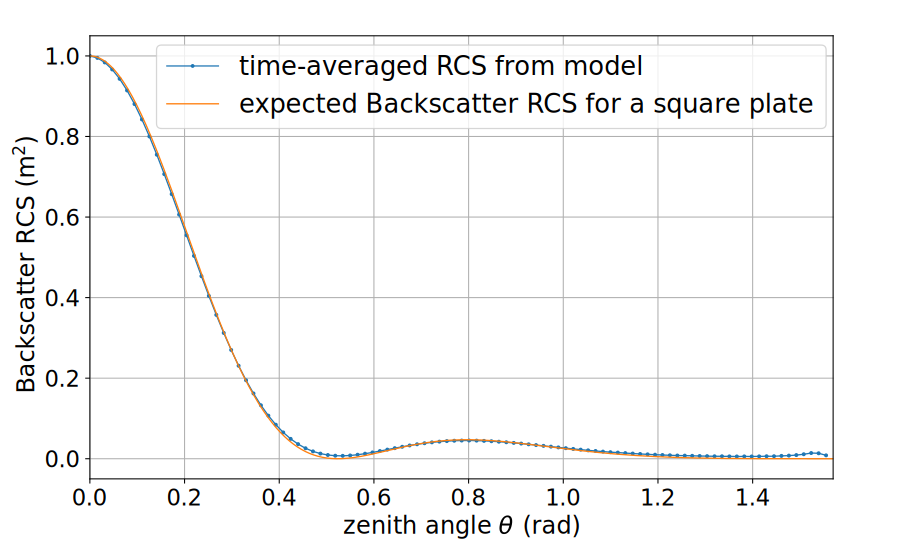
\includegraphics[width=0.8\textwidth]{images/plots/short_2D_cloud_rcs_backscatter_20lambda.pdf}
	\caption{Thin square plate monostatic backscatter. The simulated trend for the normalized RCS (in blue) follows the expected behavior (in orange) as a function of the zenith angle.}
	\label{fig:2D_cloud}
\end{figure}

\noindent The normalized RCS matches the expected behavior of a square plate. This confirms the accuracy of the code. The amplitude was not reproduced since the code is purposed for modeling a material much different from a metal: a cloud. Reproducing the movement of free electrons on a conductive plate is not the main topic of this work, but it can be done describing the electrons with the Thompson scattering cross section.

\section{Rain volumes simulations}
\label{sec:rain_volume_sims}

\noindent All simulations of this work are meant to quantify the power received from scattering by one (Section~\ref{sec:single_raindrop_results}) ore more (Section~\ref{sec:results_portion} and Section~\ref{sec:results_large}) hydrometeors suspended in the atmosphere. The geometry and power transmitted do not reproduce any specific event but are rather a representative of a generic phenomenon of hydrometeor scattering. Specific detector conditions are a topic of upcoming work. \\

\noindent Astroparticle observatories monitor the VHF and UHF spectrum ($f \in$ [30 MHz, 3 GHz]), a range shared with numerous powerful anthropogenic sources. These include FM radio stations and digital television broadcasts, which typically radiate at effective isotropic radiated powers (EIRP)\footnote{In telecommunications, the term EIRP refers to the power that would have to be radiated by an hypothetical isotropic antenna to achieve the same signal level in the direction of maximum radiation of an antenna.} of tens to hundreds of kilowatts. Airborne radars can reach 1 MW, while ground based installations often emit tens of MW. The most powerful radars on Earth are the over-the-horizon (OTH) ones, which use skywave propagation for long-range surveillance and early warning. Their typical EIRP ranges from tens of MW to over a GW. While radio and TV are continuous, narrowband sources, radars emit high-power wideband bursts with long quiet periods.\\

\noindent Within the MARES framework, the EIRP in the direction of the target, is represented by $P\text{eff}=P_{\text{T}}\times G_{\text{T}}$, where $G_{\text{T}}$ is the antenna gain, assumed one in this work. \\

\noindent We have detailed in Section~\ref{sec:final_adaptation} how, given a scattering event, parameters like the RCS and the voltage received are retrieved for each moment in time. The following results represent the average in time of these values. For a pure, unmodulated continuous wave, the average received voltage ($P_{\text{cw}}$) must exceed the noise floor of the instrument to be measurable. This is the parameter we use to estimate the detectability of hydrometeor scattering.\\

\noindent To understand or reproduce the hereby presented results one can keep in mind the following geometry:

\begin{itemize}
	\item [-] One transmitter located at the origin $(x, y, z) = (0, 0, 0)$ m;
	\item [-] One receiver positioned at increasingly larger distances from the transmitter $(x, y, z)$ =  (0 m, $y_{\text{R}}$, 0 m), tuned on the same frequency as the transmitter;
	\item [-] One target (raindrop or rain volume) suspended in the atmosphere $(x, y, x)$ =  (0 m, $y_{\text{tg}}$, 600 m).
\end{itemize}  

\noindent Without loss of generality, we make the following choices: the scattering plane is the $xy$-plane, therefore $x_{\text{tg}} = 0$ m. Furthermore, since it doesn't limit the number of scattering angles considered, the target is always positioned in the middle to simplify calculations: $\alpha = (\pi - \theta)/2$, where $\alpha$ is the angle between the vertical and $\vec{R}_{\text{T}}$, for a graphical representation, see Figure \ref{fig:geometry2}. \\

\begin{figure}[!t]
	\centering
	\includegraphics[width=0.8\textwidth]{images/geometry_2.png}
	\caption{Geometry of the simulation. The Earth's reference frame is portrayed in purple, along with two antennas and an elevated target in symmetrical position. The scattering angle $\theta$ is related to $\alpha$ according to $\alpha = (\pi - \theta)/2$.}
	\label{fig:geometry2}
\end{figure}

\noindent Target and receiver positions $y_{\text{tg}}$ and $y_{\text{R}}$ are varied from 0 to $\tan(\alpha)\cdot 600$ m and 0 to $2\tan(\alpha)\cdot 600$ m respectively, covering scattering angles $\theta \in [\pi, 0)$.

\newpage

\subsection{Results for a single raindrop}
\label{sec:single_raindrop_results}

\begin{figure}[!h]
	\centering
	\begin{subfigure}{0.7\textwidth}
		\centering
		\includegraphics[width=\textwidth]{images/plots/single_sphere_bistatic_surface_plot.pdf}
		\caption{Surface plot.}
	\end{subfigure}
	\hfill
	\begin{subfigure}{0.7\textwidth}
		\centering
		\includegraphics[width=\textwidth]{images/plots/single_sphere_bistatic_heatmap.pdf}
		\caption{Heatmap.}
	\end{subfigure}
	\caption{Radar cross section of a water sphere with $D = 1.69$ mm.}
	\label{fig:single_sphere}
\end{figure}

\noindent The MARES results for scattering from a single water sphere are represented in Figure~\ref{fig:single_sphere}. The full 3D surface plot of the $\sigma_{RCS}$ shows the angular dependency expected from theory (Figure~\ref{fig:angular_distribution}) and an absolute value consistent with the order of magnitude obtained from Equation \ref{eq:effective_area}, with size of droplet $D = 2a = 1.69$ mm and wavelength $\lambda$ = 1 m.

\newpage

\subsection{Results for a small spherical rain volume}
\label{sec:results_portion}

\begin{figure}[!h]
	\centering
	\includegraphics[width=0.7\textwidth]{images/plots/5m_sphere_heatmap_betterresolution_test2_cut.pdf}
	\caption{Radar cross section of a spherical rain volume of 5 meters radius containing raindrops with $D = 1.69$ mm and density 0.1 $\text{g}/\text{cm}^{3}$.}
	\label{fig:5m_sphere_better_resolution}
\end{figure}

\noindent A sphere of 5 m radius contains multiple raindrops. In the case of raindrops of 1.69 mm diameter we found that the density is around 40 raindrops$/\text{m}^{3}$. The response of a spherical volume of that many raindrops is depicted in Figure~\ref{fig:5m_sphere_better_resolution}. \\


\noindent For a target with dimensions comparable to the wavelength, constructive and destructive interference phenomena arise. These interference effects are highly dependent on the angular configuration, leading to a Radar Cross Section (RCS) that can either exceed or fall below that of an isolated droplet. \\

\noindent As mentioned in Section~\ref{sec:small_cloud}, the values from this plot are tabulated to be used in the next simulations (large rain volume) and overcome computational complexity.

\subsection{Results for a large rain volume}
\label{sec:results_large}

\begin{figure}
	\centering
	\begin{minipage}{0.48\textwidth}
		\centering
		\includegraphics[width=\textwidth]{images/plots/medium_cloud100_5mspheres_300MHz_heatmap_betterresolution.pdf}
		\caption{Radar cross section of a cubic cloud of 100$^{3}$ $\text{m}^{3}$.}
		\label{fig:cube_cloud100}
	\end{minipage}
	\hfill
	\begin{minipage}{0.48\textwidth}
		\centering
		\includegraphics[width=\textwidth]{images/plots/medium_cloud300_5mspheres_300MHz_heatmap_betterresolution.pdf}
		\caption{Radar cross section of a cubic cloud of 300$^{3}$ $\text{m}^{3}$.}
		\label{fig:cube_cloud300}
	\end{minipage}
\end{figure}


\begin{figure}
	\centering
	\begin{minipage}{0.48\textwidth}
		\centering
		\includegraphics[width=\textwidth]{images/plots/medium_cloud500_5mspheres_300MHz_heatmap_betterresolution.pdf}
		\caption{Radar cross section of a cubic cloud of 500$^{3}$ $\text{m}^{3}$.}
		\label{fig:cube_cloud500}
	\end{minipage}
	\hfill
	\begin{minipage}{0.48\textwidth}
		\centering
		\includegraphics[width=\textwidth]{images/plots/medium_cloud700_5mspheres_300MHz_heatmap_betterresolution.pdf}
		\caption{Radar cross section of a cubic cloud of 700$^{3}$ $\text{m}^{3}$.}
		\label{fig:cube_cloud700}
	\end{minipage}
\end{figure}

\noindent For the larger volume of rain, the shape of a cube is taken into consideration. The scattering points are placed into a three-dimensional matrix structure that extends for $L$ in all directions. Each scattering point is associated with a RCS from the table retrieved in Section~\ref{sec:results_portion}, using the procedure explained in Section~\ref{sec:big_cloud}. From Figures~\ref{fig:cube_cloud100} to~\ref{fig:cube_cloud700} the RCS of a cubic cloud with variable $L$ is presented. $L$ runs from 100 m to 700 m.\\

\noindent The RCS grows with the effective size of the cloud. The effective size being the intersection between the cloud and the beamwidth of the signal. Both of these are kept generic throughout this study. Figure~\ref{fig:sizes} represents the variation of the RCS as a function of the effective size.\\

\newpage
\begin{figure}
	\centering
	\includegraphics[width=0.7\textwidth]{images/plots/rcs_sizes_all_thetas_phi=1.5.pdf}
	\caption{Radar cross section as a function of the effective size of the rain volume. The dependence is portrayed for different values of $\theta$, and a fixed $\phi = 45^{\circ}$.}
	\label{fig:sizes}
\end{figure}

\noindent As expected, the RCS grows with the volume illuminated by the transmitter. However, the growth is limited by destructive interference phenomena within the volume. Therefore, it is expected that beyond certain critical size, further expansion of the simulated volume returns a negligible effect on the RCS. The precise determination of this threshold was precluded by prohibitive computational constraints.\\

\noindent For the following analysis, a cloud the size of 500$^{3}$ $\text{m}^{3}$ is considered, keeping in mind that in any specific case the RCS can vary by few orders of magnitude depending on the beamwidth and the height of the rain volume. \\

\noindent The analysis proceeds by fixing the angular coordinates $\theta$ and $\phi$ to isolate the dependence of the detected signal on other parameters. These are, the frequency of the signal, the distances $R_{\text{T}}$ and $R_{\text{R}}$ and the power transmitted. \\

\noindent Firstly, we notice that the only parameter that influences the RCS other than the effective size, is the frequency of the signal, therefore it is insightful to plot the reflectivity factor (RCS/Volume) as a function of frequency (see Figure~\ref{fig:RCS_freq}).\\

\begin{figure}
	\centering
	\includegraphics[width=0.7\textwidth]{images/plots/RCSlambda_5mspheres.pdf}
	\caption{Reflectivity factor of a rain volume as a function of frequency. There is a linear dependency between reflectivity and frequency in the UHF range.}
	\label{fig:RCS_freq}
\end{figure}

\noindent The reflectivity varies of two orders of magnitude along the UHF range. The choice of a specific frequency in this range changes the detected signal only by one order of magnitude at most, since the voltage received depends on $\sqrt{\sigma_{\text{RCS}}}/f$ (see Equation~\ref{eq:code_equation_voltage}).\\

\noindent In Figure \ref{fig:R1R2} is quantified the voltage received from a signal with EIRP of $10^{3}$ W at 900 MHz, scattered by a 500$^{3}$ $\text{m}^{3}$ cloud. Fixed these three variables, the voltage depends on the RCS of the target (determined by the hydrometeors' type, density and distribution) and the distances between the target and the antennas, $\text{R}_{\text{T}}$ and $\text{R}_{\text{R}}$.  \\

\begin{figure}
	\centering
	\includegraphics[width=0.6\textwidth]{images/plots/900MHz_5mspheres_R1R2.pdf}
	\caption{Reflected voltage from a 500$^{3}$ $\text{m}^{3}$ convective rain volume. A radiated signal with EIRP = $10^{3}$ W at 900 MHz is considered.}
	\label{fig:R1R2}
\end{figure}

\noindent As expected, the dependence from $\text{R}_{\text{T}}$ and $\text{R}_{\text{R}}$ is symmetric between transmitter and receiver. It is interesting to notice that the reflection is more effective when $y_{\text{tg}}$ is the middle point between the antennas ($\text{R}_{\text{T}} = \text{R}_{\text{R}}$). \\

\noindent As a rule of thumb, we consider the minimum voltage that can be significant for a typical radar system is in the order of magnitude of $\mu V$. The exact threshold for detection will greatly depend on the instrumentation and trigger method of each particular radio detector. Therefore, the analysis was constrained to ranges where $\text{R}_{\text{R}}+\text{R}_{\text{T}}<500$ km. Outside of this limit, the predicted signal strength would fall below the detectable threshold adopted here. \\

\noindent The last variable to be considered is the transmitted power, which effectively is also influenced by the gain of the transmitter antenna. The results of varying the effective power transmitted ($\text{P}_{\text{T}}\text{G}_{\text{T}}$), while keeping fixed $\text{R}_{\text{R}} = 0.5$ km are depicted in Figures~\ref{fig:PTR2_100} and~\ref{fig:PTR2_900}. \\

\begin{figure}
	\centering
	\begin{minipage}{0.48\textwidth}
		\centering
		\includegraphics[width=1\textwidth]{images/plots/100MHz_5msphere_PTR2.pdf}
		\caption{Radiated signal at 100 MHz.}
		\label{fig:PTR2_100}
	\end{minipage}
	\hfill
	\begin{minipage}{0.48\textwidth}
		\centering
		\includegraphics[width=1\textwidth]{images/plots/900MHz_5msphere_PTR2.pdf}
		\caption{Radiated signal at 900 MHz.}
		\label{fig:PTR2_900}
	\end{minipage}
	\caption{Received voltage from a 500$^{3}$ $\text{m}^{3}$ convective rain volume.}
\end{figure}

\noindent The received voltage from hydrometeor scattering is not negligible for distances between the antennas up to 500 km, admitting EIRP = 1 kW at least. This is true for both extremes of the UHF range. Another interesting remark is that the effective size of the rain volume could change the received voltage by one order of magnitude. This consideration is obtained remembering the variability of the RCS over the sizes in Figure~\ref{fig:sizes} and  the square root dependence from $\sigma_{\text{RCS}}$ in Equation~\ref{eq:code_equation_voltage}. \\

\noindent Figures from~\ref{fig:t_7_p_90} to~\ref{fig:t_180_p_90} show the variability of the received voltage with geometry. In each plot a radiated signal at 900 MHz is considered. \\

\begin{figure}
	\centering
	\begin{minipage}{0.48\textwidth}
		\centering
		\includegraphics[width=\textwidth]{images/plots/900MHz_5msphere_PTR2.pdf}
		\caption{Reflected voltage from a 500$^{3}$ $\text{m}^{3}$ rain volume. The geometry is fixed at: $\theta = 7^{\circ}$, $\phi = 90^{\circ}$.}
		\label{fig:t_7_p_90}
	\end{minipage}
	\hfill
	\begin{minipage}{0.48\textwidth}
		\centering
		\includegraphics[width=\textwidth]{images/plots/300MHz_5msphere_PTR2_t14_p90.pdf}
		\caption{Reflected voltage from a 500$^{3}$ $\text{m}^{3}$ rain volume. The geometry is fixed at: $\theta = 14^{\circ}$, $\phi = 90^{\circ}$.}
		\label{fig:t_14_p_90}
	\end{minipage}
\end{figure}


\begin{figure}
	\centering
	\begin{minipage}{0.48\textwidth}
		\centering
		\includegraphics[width=\textwidth]{images/plots/300MHz_5msphere_PTR2_t90_p90.pdf}
		\caption{Reflected voltage from a 500$^{3}$ $\text{m}^{3}$ rain volume. The geometry is fixed at: $\theta = 90^{\circ}$, $\phi = 90^{\circ}$.}
		\label{fig:t_90_p_90}
	\end{minipage}
	\hfill
	\begin{minipage}{0.48\textwidth}
		\centering
		\includegraphics[width=\textwidth]{images/plots/300MHz_5msphere_PTR2_t180_p90.pdf}
		\caption{Reflected voltage from 500$^{3}$ $\text{m}^{3}$ rain volume. The geometry is fixed at: $\theta = 180^{\circ}$, $\phi = 90^{\circ}$.}
		\label{fig:t_180_p_90}
	\end{minipage}
\end{figure}

\noindent It is possible to conclude that, if the geometry is not favorable, such as in the case of Figure~\ref{fig:t_90_p_90}, the range where hydrometeor scattering is relevant restricts to $R_{\text{T}}+ R_{\text{R}}\le 50$ km and transmitted effective power of at least 1 kW. 

	\markboth{}{} % Clear running headers
	\chapter{Final conclusions and future prospects}

\noindent For radio-based ultra-high-energy neutrino searches to succeed, possible backgrounds have to be carefully considered and understood. The radio spectrum is populated by telecommunication signals in every direction, power and frequency. Normally, these signals are easily filtrated if they are constant and well-known, but this is not always the case. \\

\noindent In the case of horizon-based signals, weather-induced variability complicates the modeling and reconstruction of signals directions. This is critical because next-generation astroparticle telescopes will target the horizon to maximize their effective volume for neutrino detection. Therefore, determining whether atmospheric effects can create unexpected detector signatures is of great importance. \\

\noindent The main focus of this thesis is evaluating the effects of a specific atmospheric propagation scenario: hydrometeor scatter, commonly associated to poor weather. Due to its transient and omnidirectional nature, the resulting signals are more difficult to distinguish from astroparticle events than fair weather phenomena. This investigation is motivated by recent evidence that atmospheric perturbation (clouds and rain) might be redirecting distant anthropogenic RFI towards detectors.\\

\noindent The approach chosen for this work is simulation-based. The computational code is a preexisting software in the field, which was adapted for this purpose. The core simulation involves a transmitter illuminating a designated volume filled with hydrometeors. These are modeled as dense particles within the Rayleigh scattering regime to simplify the physics. The code computes the scattered electromagnetic waves and, at a simulated receiver, derives key parameters like the radar cross section, received electric field and voltage. \\

\noindent As a first study of its kind, this work adopts a conceptual approach to isolate the core physical phenomenon. The simulations use a controlled, directional beam, similar to an antenna array's beamforming, to probe a specific atmospheric region. This concentrates power on a target, providing a clear measure of scattering efficiency. A full parameterization, including a detailed antenna response model, is the necessary next step, for which this work establishes the essential framework and proof of concept. \\

\noindent The received voltage was evaluated against an arbitrary but typical detection threshold of 1 $\mu V$ to identify the parameter space configurations that produce a non-negligible hydrometeor scatter signal. For quasi-forward-scatter geometries (scattering angles of $\theta = 7^{\circ} - 14^{\circ}$, the geometry corresponding to near-horizon detectors), the received voltage exceeds the threshold for total path lengths $R_{\text{T}}+R_{\text{R}}$ of up to 500 km, provided the effective transmitted power is at least 1 kW. In contrast, a more demanding geometry ($\theta=90^{\circ}$), raises the power requirement to 100 kW to produce a comparable signal in the same range. \\

\noindent In the domain of the clear-sky effects, powerful phenomena that could be evaluated in the future are are ducting, which has the potential of enhancing the transmitted signal, and reflection by the melting layer, which is theoretically more difficult to model because of the complexity of mixed-phase hydrometeors. Future work should also investigate the effects due to the ionosphere, especially sporadic E events which involve the transient presence of thin plasma capable of reflecting certain radio frequencies. \\

\noindent A valuable source to address atmospheric effects is the COST 210 \cite{ballabioCOST210Influence1991}, a report from the Commission of the European Communities. This resource provides valuable models for predicting how the atmosphere bends and focuses radio signals, creating anomalous propagation that can enhance distant terrestrial transmissions. Originally developed for telecom engineering applications, its procedures are directly applicable to radio astronomy for identifying site-specific meteorological conditions that increase vulnerability to RFI. By detailing how atmospheric effects alter a signal's angle of arrival and fading, the report enables the development of robust algorithms to veto or filter data during periods of high anomalous propagation risk. \\

\noindent This work demonstrates that reflected continuous waves (CW) from overcast skies could be detected. This poses a concern for near-horizon neutrino searches. In fact, bandwidth limitations of many radiotelescopes complicate the separation between low CW signals and astrophysical impulsive signals. Moreover, anthropogenic impulsive signals with a similar power budget are expected to represent a comparable threat too. Based on the findings presented, hydrometeor-scattered RFI cannot be ruled out as a possible source of background in radio experiments. \\

\noindent Should radio reflections from clouds be confirmed as a measurable background, near-horizon observatories will require challenging new mitigation strategies. RFI can either be non-impulsive, which includes continuous or periodic emissions from sources like oscillators and switching power supplies; or impulsive, characterized by broadband transient signals due to power line arcing and industrial sparking. The latter being distinguishable from neutrino signals only by the initial polarization and direction. Unfortunately, atmospheric effects, first and foremost hydrometeor scatter, manipulate these traits. Consequently, a likely approach is to perform a sophisticated statistical analysis that incorporates real-time meteorological data. A definitive neutrino detection from near-horizon observatories will be complex, requiring the identification of a small, isotropic excess of events against a dynamic RFI background, a process that carries significant systematic uncertainties.
	%\appendixtitleon
	%\appendixtitletocon

	\begin{appendices}
	\markboth{}{} % Clear running headers
	\chapter{The atmosphere's layers}
	\label{app:AppendixA}
	
	\section{Troposphere}
	
	\noindent The troposphere extends from the Earth's surface up to an average altitude of about 10 km. It contains 99\% of the total mass of water vapor and aerosols, making it the most dynamic and weather-active layer. Its composition is made of neutral molecules (N$_{2}$, O$_{2}$, H$_{2}$O), aerosols, and liquid or solid water droplets. The troposphere hosts electrical phenomena like thunderstorms, lightning, fair-weather electric fields, and cosmic ray ionization. It is weakly ionized, because no free electrons can survive the collisions with molecules and ions of air. The tropopause (the upper boundary of the troposphere) is marked by a temperature inversion, where cooling stops and stratospheric warming (due to ozone absorption of UV) begins. This layer acts as a "lid", trapping most weather phenomena below itself~\cite{Troposphere}.
	
	\begin{comment}
	About fair-weather electric fields. A global electric circuit exists, with thunderstorms charging the ionosphere (~300 kV potential difference between Earth and ionosphere). Even in fair weather, a weak (~100 V/m) downward electric field is present.
	\end{comment}
	
	\section{Stratosphere}
	\noindent The stratosphere is composed of stratified temperature zones, with the warmer layers of air located higher, closer to outer space, and the cooler layers below. The increase of temperature with altitude is a result of the absorption of the Sun's ultraviolet (UV) radiation by the ozone layer, where ozone is exothermically photolyzed\footnote{ Photolysis is a chemical reaction in which molecules of a chemical compound are broken down by absorption of photons.} into oxygen in a cyclical fashion~\cite{Stratosphere}.
	
	\section{Mesosphere}
	\noindent The mesosphere lies above altitude records for aircrafts, while only the lowest kilometers are accessible to balloons. At the same time, it is below the minimum altitude for orbital spacecraft due to high atmospheric drag. This region has only been accessed through the use of sounding rockets, which are only capable of taking measurements for a few minutes per mission. As a result, the mesosphere is the least-understood part of the atmosphere~\cite{Mesosphere}.
	
	\section{Ionosphere}
	
	\noindent At heights above 60 km, in the thermosphere, the atmosphere is so thin that free electrons can exist for short periods of time, before they are captured by a nearby positive ion. The number of these free electrons is sufficient to affect radio propagation. This portion of the atmosphere contains a partially ionized plasma, referred to as the ionosphere. The ionosphere and extends up to $\sim$1000 km above the sea level. The ionization is caused by several mechanisms. The rate of ionization at any altitude depends on the atmospheric composition as well as the characteristics of the incident radiation at that height. For example, as the solar radiation propagates down through the atmosphere, its various frequency (energy) bands are attenuated by different amounts. At the same time, since the composition of the atmosphere alters with altitude, different ionization processes become predominant at different heights resulting in a layered structure. The number of layers, their heights and their ionization density vary with time and space; the principal layers are three dynamic layers~\cite{Ionosphere}~\cite{barclayPropagationRadioWaves2003}. \\
	
	\begin{itemize}
		\item[-] \textbf{The D layer} is primarily responsible for absorbing low-frequency radio waves. Ionization here is due to the Lyman series-alpha radiation of hydrogen ionizing nitric oxide (NO). In this layer, higher wavelengths experience greater absorption because they move the electrons farther, leading to greater chance of collisions. This is the main reason for absorption of HF radio waves, particularly at 10 MHz and below, with progressively less absorption at higher frequencies.
		\item[-] \textbf{The E layer}, also known as the Kennelly-Heaviside layer, can reflect radio waves, allowing for long-distance communication. Ionization is due to soft X-ray (1 - 10 nm) and far ultraviolet (UV) solar radiation ionization of molecular oxygen (O$_{2}$). Normally, at oblique incidence, this layer can only reflect radio waves having frequencies lower than about 10 MHz and may contribute to absorption on frequencies above. However, during intense sporadic E events, the E$_{\text{s}}$ layer (sporadic E-layer) can reflect frequencies up to 50 MHz and higher. The E$_{\text{s}}$ layer is characterized by small, thin clouds of intense ionization. Sporadic E events may last for just a few minutes to many hours.
		\item[-] \textbf{The F layer} has the highest electron density, which implies signals that surpass this layer will escape into space. Electron production is dominated by extreme UV (10 - 100 nm) radiation ionizing atomic oxygen. The F layer consists of one layer (F2) at night, but, during the day, a secondary peak (labeled F1) often forms in the electron density profile. Because the F2 layer remains by day and night, it is responsible for most sky-wave propagation of radio waves and long distance high frequency (HF) radio communications.
	\end{itemize}
	
	\markboth{}{} % Clear running headers
	\chapter{Ducting propagation}
	\label{app:AppendixB}	
	
	\noindent For heights much less than the scale height ($H \simeq 8$ km), the exponential in Eq. \ref{eq:exponential_N} can be approximated by:
	
	\begin{equation}
		N = N_{s} (1 - \frac{z}{H}),
	\end{equation}
	
	\noindent giving a linear decrease of refractivity with height at a rate of about 40 N units per kilometer at mid latitudes. \\
	
	\noindent It can be shown that the radius of curvature, C, of a ray is very well approximated by
	
	\begin{equation}
		C = -\frac{dn}{dz}
	\end{equation}
	
	\noindent at low elevation angles. The curvature of the earth is $1/a$ where $a$ is the Earth’s radius (approximately 6378 km). Thus the curvature of the ray relative to the curvature of the Earth is 
	
	\begin{equation}
		C_{\text{relative}} = -\frac{dn}{dz}-\frac{1}{a},
	\end{equation}
	
	\noindent with 
	
	\begin{equation}
		\frac{1}{a} = 157 \times 10^{-6} \, \text{km}^{-1}.
	\end{equation}
	
	\noindent Since we are often mainly interested in this relative curvature, it is useful to introduce the concept of an effective Earth's radius $a_{\text{eff}} = ka$.\\
	
	\noindent Then we have:
	
	\begin{equation}
		C_{\text{relative}} = -\frac{dn}{dz}-\frac{1}{a} = -\frac{dn_{\text{eff}}}{dz} - \frac{1}{a_{\text{eff}}}
	\end{equation}
	
	\noindent where $n_{\text{eff}}$ is the effective refractive index associated with the effective Earth's radius.\\
	
	\noindent Note that the curvature of Earth substantially exceeds the downward curvature of the ray. in fact, in the average mid-latitude atmosphere:
	
	\begin{equation}
		C = -\frac{dn}{dz} = -\frac{dN}{dz} 10^{-6} = -40 \times 10^{-6}\,\text{km}^{-1}.
	\end{equation}\\
	
	\noindent Straight line ray propagation relative to the effective Earth's radius can then be arranged by setting $\frac{dn_{\text{eff}}}{dz} = 0$, which leads to: $\frac{1}{a_{\text{eff}}} = 117 \times 10^{-6} \, \text{km}^{-1}$, corresponding to a k factor $k = 4/3$. \\
	
	\noindent This is a well known Earth's radius construction, useful in engineering calculations. A ray propagating in a straight line over terrain based on a 4/3 effective Earth's radius is equivalent to a ray propagating in an atmosphere with the average lapse rate (the gradient of the refractivity index with height) of 40 N km$^{-1}$ over the actual terrain. For terrestrial radio links, it is a simple matter to check for terrain clearance or obstruction by joining potential transmitter and receiver positions by straight lines on 4/3 Earth-radius graph. \\
	
	\noindent There is a third viewpoint, useful in ducting studies: replacing the Earth with a flat one ($k = \infty $) and modify the curvature of the ray so that the relative curvature between ray and earth is preserved. In this case $n_{\text{eff}}$ and $N$ are replaced by the modified refractive index $m$, and the modified refractivity $M$.
	
	\begin{equation}
		M = N + 10^{6} \times z/a = N + 157 z
	\end{equation}
	
	\noindent Where $z$ is given in kilometers. \\
	
	\noindent Note that rays curve upwards relative to a flat earth:
	
	\begin{equation}
		\frac{\partial M}{\partial z} = \frac{\partial N}{\partial z} + 157.
	\end{equation}\\
	
	\noindent Although $N$ decreases by about 40 N km$^{-1}$ (M increases by about 117 N km$^{-1}$) in average conditions at mid latitudes in the lower troposphere, significant deviations from the average do occur. Figure \ref{fig:refraction} shows schematically the classification of different refractive conditions.
	
	\begin{figure}[!h]
		\centering
		\includegraphics[width=0.8\textwidth]{images/refraction.png}
		\caption{Classification of refractive conditions. If the lapse rate of $N$ is less than 40 N km$^{-1}$, the downward curvature of radio rays will decrease, shortening the radio horizon and reducing the clearance above terrain on terrestrial paths; this is known as subrefraction. On the other hand, if the lapse rate of $N$ exceeds 40 N km$^{-1}$, the ray curvature will increase, extending the radio horizon and increasing path clearance; this is known as superrefraction.}
		\label{fig:refraction}
	\end{figure}

	\noindent When the lapse rate of N exceeds 157 N km$^{-1}$, or equivalently, $\frac{\partial M}{\partial z} < 0$, then the rays are bent towards the Earth more rapidly than the Earth’s curvature. Consequently, the radio wave is no longer just bending, it's being trapped and reflected repeatedly between an upper and lower boundary. This is known as ducting and can cause rays to propagate to extremely long ranges beyond the normal horizon.\\
	
	\noindent The sensitivity of $N$ to variations in the meteorological parameters can be found by differentiating Eq. \ref{eq:refractivity}:
	
	\begin{equation}
		\delta N = 0.26 \delta P + 4.3 \delta e - 1.4 \delta T.
	\end{equation}
	
	\noindent The vertical pressure gradient $ \delta P$ never deviates much from its standard value, while differences of a few degrees in $T$ and a few millibars in $e$ can occur between adjacent air masses in certain meteorological conditions. This can lead to changes of several tens of N units over a height interval of tens of meters, and the formation of a ducting layer.\\
	
	\noindent There are two types of ducting propagation, one caused by a surface duct, the other by an elevated duct. Radio energy can become trapped between a boundary in the troposphere and the surface of Earth or sea (surface duct), or between two boundaries in the troposphere (elevated duct). With this trapped propagation, very high signal strengths can be obtained at very long range (far beyond line of sight). Indeed, the signal strength may well exceed its free space value. \\
	
	\noindent Equation \ref{eq:refractivity} shows that two processes can cause the formation of high lapse rates: a rapid decrease in water vapor pressure with height, and an increase in temperature with height (a temperature inversion); these mechanisms often occur together.
	
	\noindent A ducting layer is immediately identifiable by a negative slope in the modified refractivity versus height curve, therefore three distinct duct types exist (see Figure \ref{fig:duct_types}).\\

	\begin{figure}[!h]
		\centering
		\begin{minipage}{0.5\textwidth}
			\begin{itemize}
				\item[(a)] \textbf{Surface layer, surface duct}: The critical inversion or refractivity gradient is ground-based. The duct forms entirely within the surface layer (e.g. 100 - 200 m).
				\vspace{3cm}
				\item[(b)] \textbf{Elevated layer, surface duct}: An inversion layer exists aloft (e.g., at 500 m altitude), but its influence extends down to the surface.
				\vspace{3cm}
				\item[(c)] \textbf{Elevated layer, elevated duct}: The M-profile has a local minimum aloft, trapping waves without reaching the surface. The entire duct is suspended above the surface (e.g., 500 - 1000 m).
			\end{itemize}
		\end{minipage}%
		\begin{minipage}{0.7\textwidth}
			\includegraphics[width=0.5\linewidth]{images/ducts.png}
		\end{minipage}
		\caption{Classification of atmospheric duct types showing (a) surface-based duct, (b) elevated-layer surface duct, and (c) elevated duct, with their characteristic modified refractivity height profiles. Figure taken from~\cite{barclayPropagationRadioWaves2003}. }
		\label{fig:duct_types}
	\end{figure}
	
	\noindent Both types of surface duct are seen to propagate energy well beyond the normal radio horizon. However, a ducting layer will only trap radio waves if certain geometrical constraints apply. In particular, the angle of incidence at the layer must be very small. A simple rule of thumb can be derived from the total-internal reflection condition of geometrical optics. That is, the maximum angle of incidence $\theta_{\text{max}}$ (in degrees) is related to the change in refractivity $\Delta N$ (in N units) across the layer by:  
	
	\begin{equation}
		\theta_{\text{max}} = 0.081 \sqrt{\left | \Delta N  \right | }   
	\end{equation}
	
	\noindent As $\Delta N$ rarely exceeds 50 N units, $\theta_{\text{max}}$ will be limited between 0.5$^{\circ}$ - 1$^{\circ}$. Simple geometrical considerations show that even energy launched horizontally will intercept an elevated layer at a nonzero angle due to the Earth’s curvature. It follows that ducting layers higher than about 1 km will not significantly affect terrestrial radio links.
	
	\markboth{}{} % Clear running headers
	\chapter{Attenuation of electromagnetic waves}
	\label{app:AppendixC} 
	
	\noindent The electric and magnetic fields propagating in a lossless medium can be written like:
	
	\begin{equation}
		\vec{E}(\vec{r}, t) = \Re\left( E_{0}e^{-i(\vec{k}\cdot \vec{r} - \omega t + \varphi)}  \right) \hat{E} = E_{0}cos\left(- \vec{k}\cdot \vec{r} + \omega t - \varphi \right) \hat{E}
	\end{equation}
	
	\begin{equation}
		\vec{B}(\vec{r}, t) = \frac{1}{c}\left(\vec{k}\times \vec{E}(\vec{r}, t)\right)
	\end{equation}
	
	\noindent where $E_{0}$ is the amplitude of the electric field, $\hat{E}$ is the polarization versor and $\vec{k}$ is the direction of propagation of the electromagnetic wave. $\omega$ is the angular frequency $\omega = 2 \pi \nu$ and $\varphi$ is the free phase of the wave. \\
	
	\noindent No medium except vacuum is lossless, there are a number of physical mechanisms that will interfere with the electromagnetic wave when traveling through a real medium. Depending on the medium and wavelength, the effects of some of these phenomena cannot be neglected. Since any diffraction or refraction due to terrain and atmospheric irregularities has been neglected in this work, only polarization effects and extinction through the medium will be considered.
	
	\section{Extinction}
	\label{app:AppendixC.1} 
	\noindent Extinction generates an attenuation in wave intensity due to combined absorption and scattering. \\
	
	\noindent To take into account possible extinction losses we need to reach an equation for $\vec{E}(\vec{r}, t)$ where $E_{0}=E_{0}(r)$. This is obtained by representing the coefficient $\beta$ as the imaginary component of the wave vector $\vec{k}$, ($\vec{k} = \vec{k}_{0} - i\beta$). Therefore the wave equation is:
	
	\begin{equation}
		\begin{split}
			\vec{E}(\vec{r}, t) &= \Re\left( E_{0}e^{-i([\vec{k}_{0} - i\beta]\cdot \vec{r} - \omega t + \varphi)} \right) \hat{E} \\
			&= E_{0}e^{-r\beta} \cos\left( -\vec{k}\cdot \vec{r} + \omega t - \varphi \right) \hat{E} = \vec{E}(\vec{r}, t)\text{\Large$\tau$}(r, \beta)
		\end{split}
	\end{equation}
	
	\noindent $\text{\Large$\tau$}(r, \beta)$ is the ratio between the amplitude of a wave after it has traveled a distance $\Delta r$:
	
	\begin{equation}
		\text{\Large$\tau$}(r, \beta) = \frac{E(r + \Delta r, t)}{E(r, t)} = e^{-\Delta r \beta}
	\end{equation}
	
	\noindent also called transparency. If $\beta = 0$, $\vec{k}$ is real and $\text{\Large$\tau$} = 1$ , describing a fully transparent medium. \\
	
	\noindent When the transparency was first described, it was through the measurements of absorption of light of different media. Nowadays it is written in terms of the radiant power $P$:
	
	\begin{equation}
		P (\Delta r) = \frac{dQ_{e}(\Delta r)}{dt} = P_{0} e^{-\Delta r \gamma} = P_{0}\eta_{\text{att}}(\Delta r, \gamma)
	\end{equation}
	
	\noindent where $\eta_{\text{att}}$ is the attenuation efficiency, and $\eta_{\text{att}} < 1 \hspace{0.1cm} \forall \hspace{0.1cm} \gamma > 1$.\\
	
	\noindent The average radiant energy is:
	
	\begin{equation}
		<Q_{e}> = \frac{1}{2} \epsilon_{0}E^{2}_{0} V   
	\end{equation}
	
	\noindent where $\epsilon_{0}$ is the free space permittivity, and $V$ is the volume occupied by the wave. Then, since $P\propto E^{2}$, we obtain that $\gamma = 2\beta$:
	
	\begin{equation}
		\gamma = - \frac{1}{\Delta r} \text{ln}\left(\frac{P (\Delta r)}{P_{0}} \right)= - 2\frac{1}{\Delta r} \text{ln} \left(\frac{E (\Delta r)}{E_{0}}\right) = 2 \beta.
	\end{equation}
	
	\noindent Since $[\gamma]$ = m$^{-1}$, we can define a characteristic distance that is the inverse of it, called attenuation length:
	
	\begin{equation}
		L_{\text{att}} = \gamma ^{-1} \rightarrow \eta_{\text{att}} = e^{-r/L_{\text{att}}}.
	\end{equation}
	
	\section{Polarization effects}
	\label{app:AppendixC.2}
	
	\noindent If the polarization of the incoming radiation does not match that of the antenna, the performance of the antenna is reduced, and the received power decreases. \\
	
	\noindent This is taken into account by the polarization loss factor $\eta_{\text{PLF}}$. This factor quantifies the power loss due to polarization mismatch between the incoming wave and the antenna's polarization. It therefore is given by:
	
	\begin{equation}
		\eta_{\text{PLF}} = \left|\hat{\rho}_{w} \cdot \hat{\rho}_{a}\right|^{2}
	\end{equation}
	
	\noindent where $\hat{\rho}_{w}$ is the polarization versor of the incoming wave and $\hat{\rho}_{a}$ the polarization versor of the antenna.\\
	
	\noindent If the wave and antenna are co-polarized (perfectly matched), $\eta_{\text{PLF}} = 1$. If they are cross-polarized (orthogonal), $\eta_{\text{PLF}} = 0$. \\
	
	\noindent To evaluate $\eta_{\text{PLF}}$ in a system that involves not only two antennas but a reflecting target in between, the contribution of the target to the polarization vector must be analyzed too. In this work a target that corresponds to the collection of multiple particles has been considered perfectly reflecting in this sense, meaning that they don't affect the polarization of the wave. \\
	
	\noindent For a target that reflects perfectly an incoming wave, the vector component of the polarization perpendicular to the scattering plane is conserved, while the one parallel to the scattering plane is rotated by 90$^{\circ}$. This description is represented in Figure \ref{fig:polarization} for better understanding. 
	
	\newpage
	
	\begin{figure}[!ht]
		\centering
		\includegraphics[width=0.9\textwidth]{images/reflection.png}
		\caption{Polarization vectors before and after reflection from target, in the assumption of perfectly reflecting target. The parallel component of the polarization vector is rotated of 90$^{\circ}$ while the perpendicular component is conserved.}
		\label{fig:polarization}
	\end{figure}
	
	\noindent In this work, for any simulation, transmitter and receiver are always considered to have the same polarization angle $\epsilon_{\text{T}} = \epsilon_{\text{R}}$, measured in the wave frame starting from $\hat{Y}_{\text{w}}$ and rotating counterclockwise from the point of view of the antenna. \\
	
	\noindent Attention must be paid to the fact that with these assumptions $\eta_{\text{PLF}} = 1$ for any geometry between target and detection system.
	
\end{appendices}
	\markboth{}{} % Clear running headers
 	\printbibliography[title=Bibliography]
	
\end{document}
